\section{Checkpointing Protocols}

\def\smiley{\green{\larger[2]\wasyfamily\char44}\xspace}
\def\frownie{\blue{\larger[2]\wasyfamily\char47}\xspace}
\def\quesley{\yyellow{\hbox to -0.08em{\textraiseglotstop}$_{\textrm{\wasyfamily\char47}}$}\xspace}

\newtheorem{proposition}{Proposition}
%\newtheorem{corollary}{Corollary}
%\newtheorem{definition}{Definition}
%\newtheorem{remark}{Remark}

%% Macros - hierarchical paper
\newcommand{\wastecoordnofail}{\ensuremath{\textsc{Waste}_{\mathit{coord-nofailure}}}}
\newcommand{\wastecoordfail}{\ensuremath{\textsc{Waste}_{\mathit{coord-failure}}}}
\newcommand{\overheadcoordfail}{\ensuremath{\Overhead_{\mathit{coord}}}}
\newcommand{\wastecoordfailinw}{\ensuremath{\textsc{Waste}_{\mathit{coord-fail-in-work}}}}
\newcommand{\overheadcoordfailinw}{\ensuremath{\Overhead_{\mathit{coord-fail-in-work}}}}
\newcommand{\wastecoordfailinc}{\ensuremath{\textsc{Waste}_{\mathit{coord-fail-in-checkpoint}}}}
\newcommand{\overheadcoordfailinc}{\ensuremath{\Overhead_{\mathit{coord-fail-in-checkpoint}}}}
\newcommand{\wastecoord}{\ensuremath{\textsc{Waste}_{\mathit{coord}}}}
\newcommand{\wckpt}{\textsc{waste}_{ckpt}}
\newcommand{\ockpt}{\Overhead_{ckpt}}
\newcommand{\ocomp}{\Overhead_{comp}}
\newcommand{\wbckpt}{\textsc{waste}_{before\_ckpt}}
\newcommand{\obckpt}{\Overhead_{before\_ckpt}}
\newcommand{\wdckpt}{\textsc{waste}_{during\_ckpt}}
\newcommand{\odckpt}{\Overhead_{during\_ckpt}}
\newcommand{\wackpt}{\textsc{waste}_{after\_ckpt}}
\newcommand{\oackpt}{\Overhead_{after\_ckpt}}
\newcommand{\avgwckpt}{\textsc{avg\_waste}_{ckpt}}
\newcommand{\avgockpt}{\textsc{avg\_\Overhead}_{ckpt}}
\newcommand{\qmin}{\ensuremath{\text{q}_{\min}}\space}%cpu frequency
\newcommand{\StenTwo}{\textsc{2D-Stencil}\xspace}
\newcommand{\StenThree}{\textsc{3D-Stencil}\xspace}
\newcommand{\Matprod}{\textsc{Matrix-Product}\xspace}
\newcommand{\CSCI}{\textsc{Coord-IO}\xspace}
\newcommand{\CSHI}{\textsc{Hierarch-IO}\xspace}
\newcommand{\CSHIPlane}{\textsc{Hierarch-IO-Plane}\xspace}
\newcommand{\CSHILine}{\textsc{Hierarch-IO-Line}\xspace}
\newcommand{\CSCP}{\textsc{Coord-Port}\space}
\newcommand{\CSHP}{\textsc{Hierarch-Port}\xspace}
\def\PP{\mathbb{P}}
\newcommand{\Topt}{\mathbb{T}^*}
\newcommand{\XX}{C}
\newcommand{\Work}{\textsc{Work}}
\newcommand{\Overhead}{\textsc{Re-Exec}}
\newcommand{\Waste}{\textsc{Waste}}
\newcommand{\Useful}{\textsc{UsefulFraction}}
\newcommand{\coord}{\text{coord}}
\newcommand{\hierarch}{\text{hierarch}}
\newcommand{\cmem}{C_{\text{Mem}}}
\newcommand{\Wastecoordopt}{{\Waste_{coord}}^*}
\newcommand{\ngroups}{\ensuremath{G}\xspace} %Number of groups in platform
\newcommand{\nsubgroups}{\ensuremath{H}\xspace} %Number of sub-groups in a group for port-saturated
\newcommand{\vgroups}{\ensuremath{g}\xspace} %Variable to iterate on groups
\newcommand{\muplatform}{\ensuremath{\mu}\xspace} %MTBF of platform
\newcommand{\nprocess}{\ensuremath{p_{total}}\xspace} %Number of processors in platform
\newcommand{\nprocessR}{\ensuremath{N}\xspace} %Number of processors in platform
\newcommand{\vsegment}{\ensuremath{s}\xspace} %Variable to iterate on segments
\newcommand{\nq}{\ensuremath{q}\xspace} %Number of processors in a group
\newcommand{\cplatform}{\ensuremath{C}\xspace} %checkpoint de la platforme
\newcommand{\rplatform}{\ensuremath{R}\xspace} %recovery de la platforme
\newcommand{\dplatform}{\ensuremath{D}\xspace} %downtime de la platforme
\newcommand{\cgroup}{\ensuremath{C(\nq)}\xspace} %checkpoint d'un groupe
\renewcommand{\rgroup}{\ensuremath{R(\nq)}\xspace} %recovery d'un groupe
\newcommand{\dgroup}{\ensuremath{D(\nq)}\xspace} %downtime d'un groupe
\newcommand{\W}{\ensuremath{W}\xspace}% travail utile
\newcommand{\T}{\ensuremath{T}\xspace} % 'Checkpoint' interval
\newcommand{\amountlog}{\ensuremath{\beta}\xspace}%Amount of logging per time unit
\newcommand{\workduringckpt}{\ensuremath{\alpha}\xspace}%Ratio of the checkpointing time that can be used as work
\newcommand{\cgroupbase}{\ensuremath{C_0(\nq)}\xspace}%Time to save the group without message logging
\newcommand{\dgroupbase}{\ensuremath{D_0(\nq)}\xspace}%Time to save the group without message logging
\newcommand{\rgroupmin}{\ensuremath{R_0(\nq)}\xspace}%Time to recover the group without message logging
\newcommand{\rgroupbase}{\ensuremath{R_0(\nq)}\xspace}%Time to save the group without message logging
\newcommand{\MFPA}{\ensuremath{\text{Mem}}\xspace}%memory footprint
\newcommand{\bwio}{\ensuremath{\text{b}_{io}}\xspace}%i/o bandwidth
\newcommand{\bwnode}{\ensuremath{\text{b}_{port}}\xspace}%inode/port bandwidth
\newcommand{\speed}{\ensuremath{\text{s}_{p}}\xspace}%cpu frequency

\newcommand{\opt}{\ema{{\text{opt}}}}
%% Macros - prediction
\newcommand{\C}{C\xspace}
\newcommand{\CC}{C\xspace}
\newcommand{\D}{D\xspace}
\newcommand{\R}{R\xspace}
\newcommand{\p}{p\xspace}
\newcommand{\q}{q\xspace}
\newcommand{\qopt}{q_{opt}}
\newcommand{\recall}{\ensuremath{r}\xspace}
\newcommand{\precision}{\ensuremath{p}\xspace}
\newcommand{\trust}{\ensuremath{q}\xspace}
\newcommand{\muP}{\ensuremath{\mu_{P}}\xspace}
\newcommand{\muNP}{\ensuremath{\mu_{NP}}\xspace}
\newcommand{\munew}{\ensuremath{\mu_e}\xspace}
\newcommand{\period}{\ensuremath{T}\xspace}

%% Macros - Dounia FTXS
\def\e{\mathop{\rm e}\nolimits}
\def\pr{\mathop{\rm Pr}\nolimits}
\def\P{\mathop{\mathbb{P}}\nolimits}
\def\E{\mathop{\mathbb{E}}\nolimits}
\def\En{\mathop{\mathbb{E}_n}\nolimits}
\def\Ew{\mathop{\mathbb{E}_w}\nolimits}
\def\EW{\mathop{\mathbb{E}_W}\nolimits}
\def\ET{\mathop{\mathbb{E}_T}\nolimits}
\def\Ep{\mathop{\mathbb{E}_p}\nolimits}
\def\Eo{\mathop{\mathbb{E}_o}\nolimits}
\def\EO{\mathop{\mathbb{E}_O}\nolimits}
\def\Eopt{\mathop{\mathbb{E}_{opt}}\nolimits}
\def\Wopt{\mathop{W_{opt}}\nolimits}
\def\Elost{\mathop{\mathbb{E}_{lost}}\nolimits}
\def\iid{\textit{iid}\xspace}
\def\Psucc{\mathop{\mathcal{P}_{\text{succ}}}\nolimits}
\def\Ewasted{\mathop{\mathbb{E}_{\text{wasted}}}\nolimits}
\def\Ewastedp{\mathop{\mathbb{E}_{\text{wasted}}}\nolimits}
\def\Topt{\ensuremath{T_{\text{opt}}}}
\def\Tcand{\ensuremath{T_{\text{cand}}}}
\def\Xp{\ensuremath{X^{(p)}}}
\newcommand{\pused}{p_{used}}
\newcommand{\Petasc}{Petascale}
\newcommand{\Exasc}{Exascale}
\newcommand{\nbfail}{n^{fail}}
%\newcommand{\s}{s}
\newcommand{\Speedup}{\mathit{loss}}
\newcommand{\Psuc}{P_{suc}}
\newcommand{\Xexec}{T}
\newcommand{\Xwork}{W}
\newcommand{\Xlost}{T_{lost}}
\newcommand{\Rlost}{R_{lost}}
\newcommand{\Xrec}{T_{rec}}
\newcommand{\Xwasted}{T_{wasted}}
\newcommand{\f}{f}
\newcommand{\talive}{\tau}
\newcommand{\w}{\omega}
\newcommand{\lamb}{\mathbb{L}} %lambert function
\newcommand{\tinit}{t^{init}}
\newcommand{\myalpha}{\alpha}
\newcommand{\mybeta}{\beta}
\newcommand{\tcst}{t^{cst}}
\renewcommand{\c}{C}
\renewcommand{\r}{R}
\renewcommand{\a}{a}
\renewcommand{\d}{D}

%% Macros replication
\newcommand{\Hopt}{\ema{\mathbb{H}_{\textit{opt}}}}
\newcommand{\nbf}{\ema{n_{\text{fail}}}}
\newcommand{\MM}{\ema{M}}
\newcommand{\bb}{\ema{b}}
\newcommand{\pg}{q}
\newcommand{\N}{N}
%\newcommand{\NFTI}{\ensuremath{\mathit{NFTI}}\xspace}
\newcommand{\NFTIkf}{\ensuremath{\mathit{NFTI}^{\mathrm{ah}}}\xspace}
\newcommand{\MNFTIbase}{\ensuremath{\mathit{MNFTI}}\xspace}
%\newcommand{\MNFTI}{\ensuremath{\mathit{MNFTI}}\xspace}
\newcommand{\MNFTIkf}{\ensuremath{\mathit{MNFTI}^{\mathrm{ah}}}\xspace}
%\newcommand{\NFTIah}{\ensuremath{\mathit{NFTI}^{\mathrm{ah}}}\xspace}
\newcommand{\NFTI}{\ensuremath{\mathit{NFTI}^{\mathrm{rp}}}\xspace}
\newcommand{\TTI}{\ensuremath{\mathit{TTI}}\xspace}
%\newcommand{\MNFTIah}{\ensuremath{\mathit{MNFTI}^{\mathrm{ah}}}\xspace}
\newcommand{\MNFTI}{\ensuremath{\mathit{MNFTI}^{\mathrm{rp}}}\xspace}
\newcommand{\MTTI}{\ensuremath{\mathit{MTTI}}\xspace}
\newcommand{\MNFTIgen}{\ensuremath{\mathit{MNFTI}}\xspace}
\newcommand{\PRR}{\textsc{Process replication}\xspace}
\newcommand{\GRR}{\textsc{Group replication}\xspace}
\newcommand{\Birthday}{\textit{Birthday}}
\newcommand{\nrep}{\ensuremath{g}\xspace} %Number of replicas in process replication
\newcommand{\nprocessrep}{\ensuremath{n_{rg}}\xspace}
\newcommand{\nfail}{n_f} % Just a variable in equations, denoting number of failures so far 
\newcommand{\RG}{replica-group\xspace}
\newcommand{\RGs}{replica-groups\xspace}
\newcommand{\murep}{\ema{\mu_{\text{rep}}}}
\def\dalyO{\textsc{Daly}-$g=1$\xspace}
\def\dalyT{\textsc{Daly}-$g=2$\xspace}
\def\bestperO{\textsc{BestPeriod}-$g=1$\xspace}
\def\bestperT{\textsc{BestPeriod}-$g=2$\xspace}


\makeatletter
\renewcommand{\boxed}[1]{\textcolor{\boxcolor}{%
\tikz[baseline={([yshift=-1ex]current bounding box.center)}] \node [rectangle, minimum width=1ex,rounded corners,draw] {\normalcolor\m@th$\displaystyle#1$};}}
 \makeatother


\newcommand{\timeline}[3]{
\draw[thin, color=black,->] (#1,#3) -- (#2,#3) node[below=-0.5pt, ] {\scriptsize{Time}};
}

\newcommand{\wasteff}{\textsc{Waste}_{\text{ff}}}
\newcommand{\wastefail}{\textsc{Waste}_{\text{fail}}}
\newcommand{\Time}[1][]{\ensuremath{\textsc{Time}_{\text{#1}}}\xspace}
\newcommand{\Wastee}[1][]{\ensuremath{\textsc{Waste}_{\text{#1}}}\xspace}
%\newcommand{\T}{\ensuremath{T}\xspace}
\newcommand{\Tp}{\ensuremath{T_{\text{P}}}\xspace}
\newcommand{\Tnp}{\ensuremath{T_{\text{R}}}\xspace}
\newcommand{\I}{\ensuremath{I}\xspace}

\newcommand{\Cr}{\ensuremath{C}\xspace}
\newcommand{\Cp}{\ensuremath{C_{p}}\xspace}
\newcommand{\Nfaults}{\ensuremath{N_{faults}}\xspace}
\newcommand{\Tlost}[1][]{\ensuremath{T_{\text{lost}#1}}\xspace}
\newcommand{\Wregular}{\ensuremath{W_{\mathit{reg}}}\xspace}


\newcommand{\promode}[3]{ %coordonnees: x gauche, x droite, y
\draw[thick, color=blue] ($(#1,#3)$) --  ($(#1,#3-1.9)$);
\draw[thick, color=blue] ($(#2,#3)$) --  ($(#2,#3-1.9)$);
\draw[draw=none] ($(#1 ,#3-1.7)$) -- ($(#2,#3-1.7)$) node[midway,color=blue] {\scriptsize{Proactive mode}};
}
%
\newcommand{\regmode}[3]{
\draw[thick, color=blue] ($(#1,#3)$) --  ($(#1,#3-1.9)$);
\draw[thick, color=blue] ($(#2,#3)$) --  ($(#2,#3-1.9)$);
\draw[draw=none] ($(#1 ,#3-1.7)$) -- ($(#2,#3-1.7)$) node[midway,color=blue] {\scriptsize{Regular mode}};
}

\newcommand{\pair}{\ema{\text{Pair}}}
\newcommand{\Throughput}{\ema{\textsc{Throughput}}}
\newcommand{\ThrouStd}{\ema{\Throughput_{\text{Std}}}}
\newcommand{\ThrouRep}{\ema{\Throughput_{\text{Rep}}}}
% Macros silent errors
\newcommand{\ema}[1]{\ensuremath{#1}\xspace}
\newcommand{\mue}{\ema{\mu_{e}}}
\newcommand{\mud}{\ema{\mu_{d}}}
\newcommand{\ccc}{\ema{C}}
\newcommand{\cc}{\ema{C}}
\newcommand{\rrr}{\ema{R}}
\newcommand{\ddd}{\ema{D}}
\newcommand{\vvv}{\ema{V}}
\newcommand{\www}{\ema{w}}
\newcommand{\sss}{\ema{\mathbb{S}}}
%\newcommand{\Waste}{\ema{\textsc{Waste}}}
\newcommand{\Wasteff}{\ema{\textsc{Waste}_{\text{ff}}}}
\newcommand{\Wastefail}{\ema{\textsc{Waste}_{\text{fail}}}}
\newcommand{\Sopt}{\ema{{S}_{\text{opt}}}}
\newcommand{\Pfd}{\ema{\mathbb{P}_{\text{risk}}}}
\newcommand{\lambdae}{\ema{\lambda_{e}}}
\newcommand{\lambdad}{\ema{\lambda_{d}}}
\newcommand{\Tmin}{\ensuremath{T_{\min}}\xspace} 
%\newcommand{\Waste}{\ema{\textsc{Waste}}}
\newcommand{\Wasteopt}{\Waste[opt]}
\newcommand{\risky}{\ema{\varepsilon}}
\newcommand{\off}{\ema{o_{\text{ff}}}}
\newcommand{\fre}{\ema{f_{\text{re}}}}
\newcommand{\BalAlgo}{\ema{\textsc{Balanced\-Algo\-rithm}}}

%Aurélien
\newcommand{\sio}{\ema{s_{\text{io}}}\xspace}
\newcommand{\sre}{\ema{\sigma}\xspace}
\newcommand{\scpu}{\ema{s}\xspace}
%\newcommand{\W}[2]{\ema{W_{#1,#2}}\xspace}
\newcommand{\WIJ}{\ema{\W{i}{j}}\xspace}
\newcommand{\WV}[1]{\ema{V_{#1}}\xspace}
\newcommand{\WVV}[2]{\ema{V_{#1}(#2)}\xspace}
\newcommand{\WC}[1]{\ema{C_{#1}}\xspace}
\newcommand{\WR}[1]{\ema{R_{#1}}\xspace}
%\newcommand{\T}[2]{\ema{T_{#1,#2}}\xspace}
\newcommand{\TIJ}{\ema{\T{i}{j}}\xspace}
\newcommand{\TV}[1]{\ema{V_{#1}}\xspace}
\newcommand{\TC}[1]{\ema{C_{#1}}\xspace}
\newcommand{\TR}[1]{\ema{R_{#1}}\xspace}
\newcommand{\TLost}{\ema{T_{{lost}_{i,j}}}\xspace}
\newcommand{\TimeC}{\ema{Time_{C}^{rec}}\xspace}
\newcommand{\TCfirst}{\ema{T_{{C}_{first}}^{SF}}\xspace}
\newcommand{\TimeCre}{\ema{Time_{{C}_{re}}^{rec}}\xspace}
\newcommand{\TimeCmul}{\ema{Time_{{C}_{mul}}^{rec}}\xspace}
\newcommand{\TimeV}{\ema{Time_{V}^{rec}}\xspace}
\newcommand{\TimeVfirst}{\ema{Time_{V_{first}}^{rec}}\xspace}
\newcommand{\TimeVC}{\ema{Time_{VC}^{rec}}\xspace}
\newcommand{\TimeVCre}{\ema{Time_{{VC}_{re}}^{rec}}\xspace}
\newcommand{\TimeVCmul}{\ema{Time_{{VC}_{mul}}^{rec}}\xspace}
\newcommand{\TVCfirst}{\ema{T_{{VC}_{first}}}\xspace}
\newcommand{\TVCsec}{\ema{T_{{VC}_{sec}}}\xspace}
\newcommand{\TCre}{\ema{T_{{C}_{re}}}\xspace}
\newcommand{\TVC}{\ema{T_{{VC}_{re}}}\xspace}
\newcommand{\TCF}{\ema{T_{C}^{F}}\xspace}
\newcommand{\TCS}{\ema{T_{C}^{S}}\xspace}
\newcommand{\TVS}{\ema{T_{V}^{S}}\xspace}
\newcommand{\TVF}{\ema{T_{V}^{F}}\xspace}
\newcommand{\TCSF}{\ema{T_{C}^{SF}}\xspace}
\newcommand{\TVSF}{\ema{T_{V}^{SF}}\xspace}
\newcommand{\TVfirst}{\ema{T_{{V}_{first}}^{SF}}\xspace}
\newcommand{\ELost}{\ema{E_{{lost}_{i,j}}}\xspace}
\newcommand{\EnergyC}{\ema{Energy_{C}^{rec}}\xspace}
\newcommand{\EnergyCre}{\ema{Energy_{{C}_{re}}^{rec}}\xspace}
\newcommand{\EnergyCmul}{\ema{Energy_{{C}_{mul}}^{rec}}\xspace}
\newcommand{\ECre}{\ema{E_{{C}_{re}}}\xspace}
\newcommand{\EnergyV}{\ema{Energy_{V}^{rec}}\xspace}
\newcommand{\EnergyTotal}{\ema{Energy}\xspace}
\newcommand{\EnergyVfirst}{\ema{Energy_{V_{first}}^{rec}}\xspace}
\newcommand{\EnergyVC}{\ema{Energy_{VC}^{rec}}\xspace}
\newcommand{\EnergyVCre}{\ema{Energy_{{VC}_{re}}^{rec}}\xspace}
\newcommand{\EnergyVCmul}{\ema{Energy_{{VC}_{mul}}^{rec}}\xspace}
\newcommand{\EVCfirst}{\ema{E_{{VC}_{first}}}\xspace}
\newcommand{\EVCsec}{\ema{E_{{VC}_{sec}}}\xspace}
\newcommand{\EVC}{\ema{E_{VC}}\xspace}
\newcommand{\ECSF}{\ema{E_{C}^{SF}}\xspace}
\newcommand{\EVSF}{\ema{E_{V}^{SF}}\xspace}
\newcommand{\EIJ}{\ema{E_{i,j}}\xspace}
\newcommand{\EVfirst}{\ema{E_{{V}_{first}}^{SF}}\xspace}
\newcommand{\EV}[1]{\ema{E_{#1}^{\text{V}}}\xspace}
\newcommand{\EVV}[2]{\ema{E_{#1}^{\text{V}}(#2)}\xspace}
\newcommand{\EC}[1]{\ema{E_{#1}^{\text{C}}}\xspace}
\newcommand{\ER}[1]{\ema{E_{#1}^{\text{R}}}\xspace}
\newcommand{\pErr}[2]{\ema{p_{#1,#2}^{\text{Err}}}\xspace}
\newcommand{\pF}[2]{\ema{p_{#1,#2}^{F}}\xspace}
\newcommand{\pS}[2]{\ema{p_{#1,#2}^{S}}\xspace}
\newcommand{\lf}{\ema{\lambda^F}\xspace}
\newcommand{\ls}{\ema{\lambda^S}\xspace}
\newcommand{\la}{\ema{\lambda}\xspace}
\newcommand{\minmakespan}{\textsc{Minimizing Makespan}\xspace}
\newcommand{\minenergy}{\textsc{Minimizing Energy}\xspace}
\newcommand{\singlespeed}{\textsc{SingleSpeed}\xspace}
\newcommand{\reexecspeed}{\textsc{ReExecSpeed}\xspace}
\newcommand{\multispeed}{\textsc{MultiSpeed}\xspace}
\newcommand{\reff}{\textrm{ref}}
\newcommand{\Power}{\ema{P}\xspace}
\newcommand{\Pidle}{\ema{P_{idle}}\xspace}
\newcommand{\Pcpu}[1]{\ema{P_{cpu}(s_{#1})}\xspace}
\newcommand{\Pcpus}{\ema{P_{cpu}(s)}\xspace}
\newcommand{\Tcpu}[1]{\ema{T_{cpu}(s_{#1})}\xspace}
\newcommand{\Pio}{\ema{P_{io}}\xspace}
\newcommand{\CPT}[1]{\ema{C_{#1}}\xspace}
\newcommand{\REC}[1]{\ema{R_{#1}}\xspace}
\newcommand{\VCO}{\textsc{VC-only}\xspace}
\newcommand{\VCV}{\textsc{VC+V}\xspace}
\newcommand{\TimeVCO}{\textsc{Time-VC}\xspace}
\newcommand{\TimeVCV}{\textsc{Time-VC+V}\xspace}
\newcommand{\EnergyVCO}{\textsc{Energy-VC}\xspace}
\newcommand{\EnergyVCV}{\textsc{Energy-VC+V}\xspace}
%\newcommand{\Topt}{\ema{T_{opt}(s)}\xspace}
\newcommand{\WA}{\ema{\text{Waste}}\xspace}


\newcommand{\distrib}{\ema{\mathcal{D}}}
\newcommand{\expo}{\ema{\textsc{Exp}}\xspace}
\newcommand{\weib}{\ema{\textsc{Weibull}}\xspace}
\newcommand{\wdaly}{\ema{W_{\textit{YD}}}\xspace}



%uncertainty
\newcommand{\mupp}{\ema{\mu_{p}}\xspace}
\newcommand{\pdaly}{\ema{T_{\textit{YD}}}\xspace}

%Uncertainty - interference
\newcommand{\nocoop}{\emph{Oblivious}\xspace}
\newcommand{\fifoblock}{\emph{Ordered}\xspace}
\newcommand{\fifononblock}{\emph{Ordered-NB}\xspace}
\newcommand{\leastwaste}{\emph{Least-Waste}\xspace}



\frame{
  \frametitle{Checkpointing Protocols}

  \begin{columns}
    \begin{column}{.45\linewidth}
      \begin{center}
        Rollback-Recovery in MPICH-V\\
        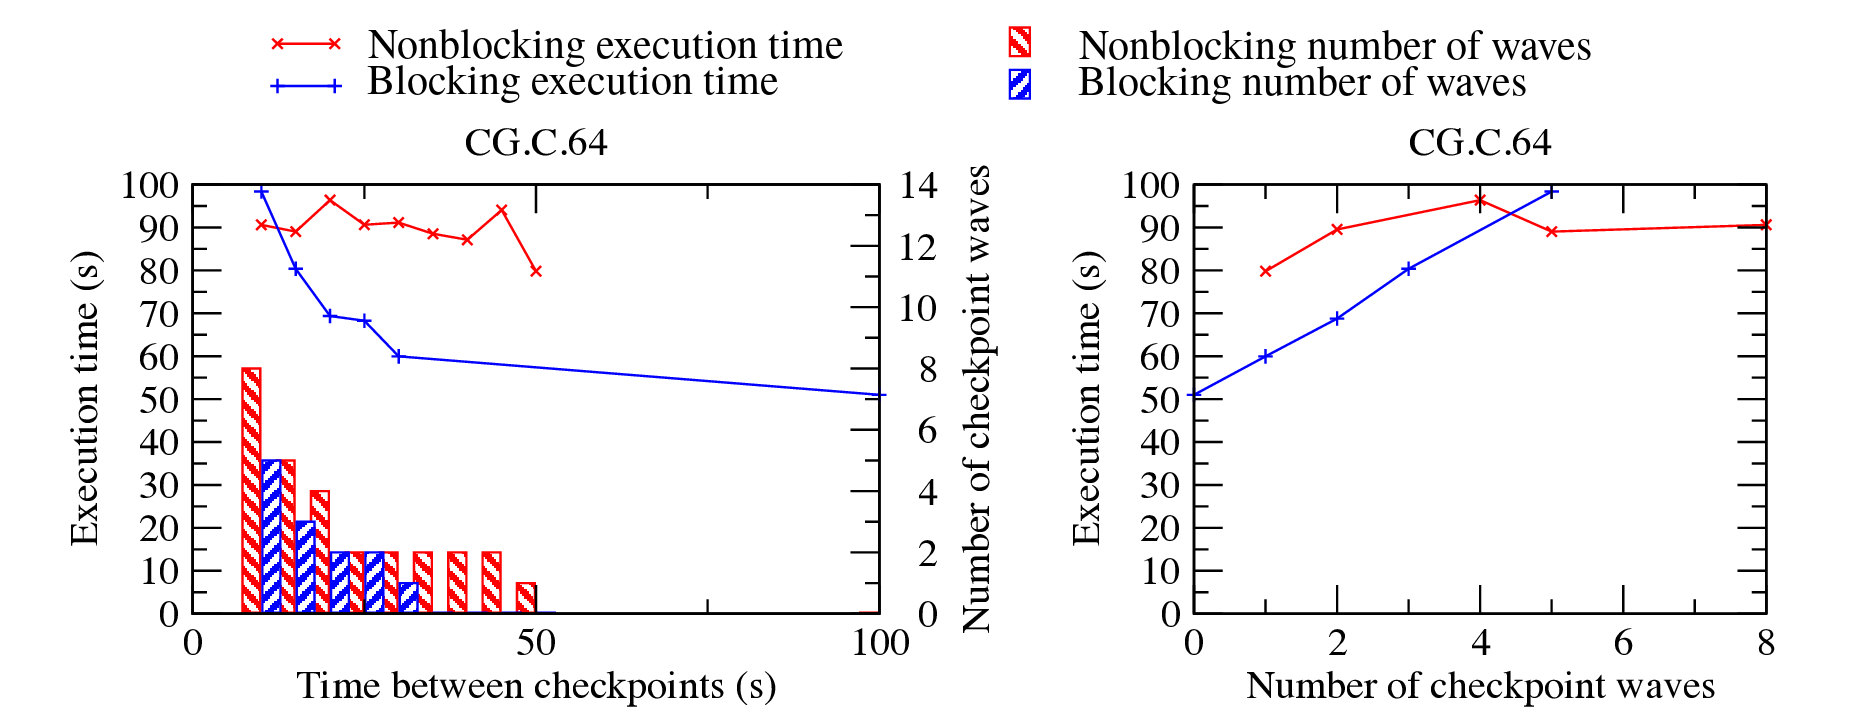
\includegraphics[width=\linewidth]{figures/mpichv-coordinated.png}\\
        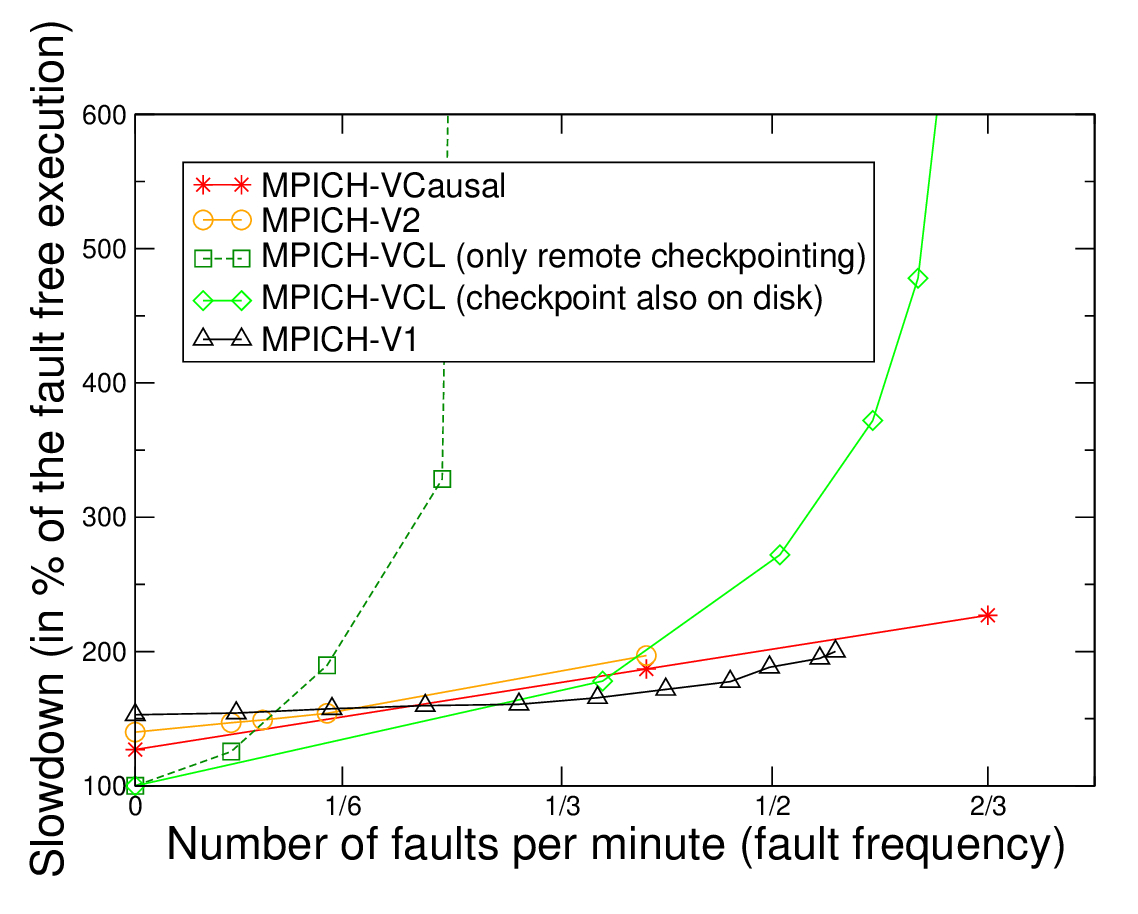
\includegraphics[width=.75\linewidth]{figures/mpichv-noncoordinated.jpg}
      \end{center}
    \end{column}
    \begin{column}{.45\linewidth}
      \begin{itemize}
      \item MPICH-V: studied experimentally rollback-recovery protocols in a Message Passing Interface library (MPICH)
      \item Subject: how to checkpoint efficiently
        \begin{itemize}
        \item Coordinated protocols (blocking, non-blocking)
        \item Uncoordinated protocols (Optimistic, Pessimistic, Causal)
        \end{itemize}
      \item Uncovered: when to checkpoint
      \end{itemize}
    \end{column}
  \end{columns}  
}

\begin{frame}
  \frametitle{Periodic checkpointing}

\begin{center}
  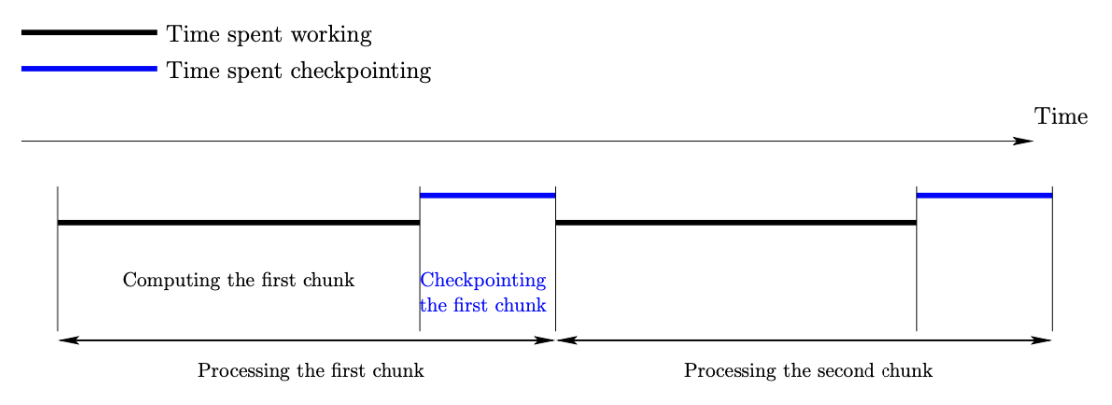
\includegraphics[width=.9\textwidth]{PeriodicCoordinatedCkpt.png}%
 \end{center}

\textbf{Blocking model:} while a checkpoint is taken, no computation can be performed
  
\end{frame}

%% \begin{frame}
%%   \frametitle{Waste in failure-free execution}

%% \vfill
%% \centering
%% \begin{tabular}{cc}
%% \begin{minipage}{.55\textwidth}
%%  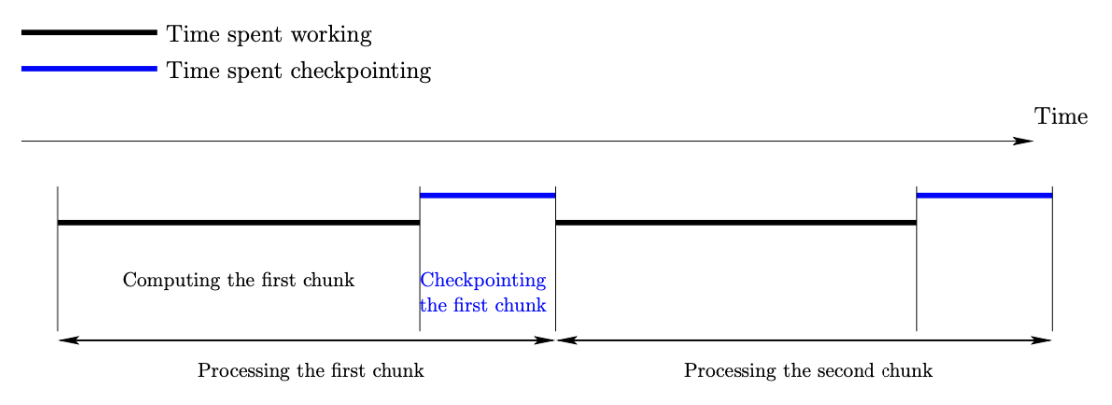
\includegraphics[width=\textwidth]{PeriodicCoordinatedCkpt.png}
%% \end{minipage}
%% &
%% \begin{minipage}{.65\textwidth}
%% \begin{itemize}
%%       \item  \Time[base]: application base time
%%        \item \Time[FF]: with periodic checkpoints\\
%%        but failure-free
%%  \end{itemize}
%%  \end{minipage}
%%  \end{tabular}
 
%% $$\Time[FF]  =  \Time[base] + \#checkpoints \times \Cr$$
%% $$\#checkpoints  = 
%% \left\lceil\frac{\Time[base]}{\period-\Cr}\right\rceil
%% \sim \frac{\Time[base] }{\period-\Cr} \text{ (valid for large jobs)}$$

%% \red{$$\Waste[FF] = \frac{\Time[FF]-\Time[base]}{\Time[FF]} = \frac{\Cr}{\period}$$}

%% \end{frame}

%% \begin{frame}
%%     \frametitle{Waste due to failures}
    
%% \begin{center}
%% 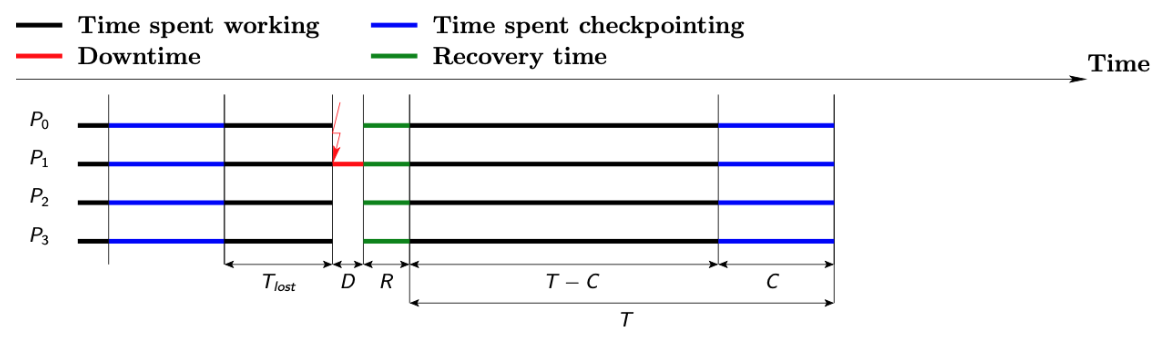
\includegraphics[width=0.95\textwidth]{NewYvesCoordinated.png}
%% \end{center}
%% $$\Tlost= \D+\R+ \frac{\period}{2}$$
  
%% \red{$$\Waste[fail] = \frac{1}{\mu} \left( \D + \R + \frac{\period}{2} \right)$$}


%% \end{frame}

%% \begin{frame}
%%   \frametitle{Total waste}
 
%% \centering
%% \centering
\begin{tikztimingtable}[
    timing/slope=0,         % no slope
    timing/rowdist=\ttrd,     % row distance
    timing/coldist=2pt,     % column distance
    xscale=3,yscale=1.5, % scale diagrams
    semithick ,              % set line width
  ]

 & G1.2D{\T-\C}G{[fill=black!20] 0.2D{\C}G}1.2D{\T-\C}G{[fill=black!20] 0.2D{\C}G}1.2D{\T-\C}G{[fill=black!20] 0.2D{\C}G}1.2D{\T-\C}G{[fill=black!20] 0.2D{\C}G}1.2D{\T-\C}G{[fill=black!20] 0.2D{\C}G}{[fill=black!80] 3DG}\\
\extracode
%  \tableheader{Probability}{\waste}
 \makeatletter
 \begin{pgfonlayer}{background}
%Ligne 0
%\arrowtime{0}{9.5};
\legende{0,0}{7}{\Time[FF]=\Time[Final](1-\Waste[Fail])};
%\legende{3.2,0}{0.9}{\Wregular};
%\legende{4.6,0}{1.1}{\T-\Wregular-\C};
\legende{7,0}{3}{$\Time[Final]\times\Waste[Fail]$};
\legende{0,-1.6}{10}{\Time[Final]};
 \end{pgfonlayer}
\end{tikztimingtable}%



%% $$\Waste= \frac{\Time[final]-\Time[base]}{\Time[final]}$$
%% $$1 - \Waste = (1-\Waste[FF])(1-\Waste[fail])$$

%% \red{$$\Waste = \frac{\Cr}{\period} + \left( 1 -  \frac{\Cr}{\period} \right) 
%% 	\frac{1}{\mu} \left( \D + \R + \frac{\period}{2} \right)$$}
%% \end{frame}

%% \begin{frame}
%%   \frametitle{Waste minimization}
 

%% $$\Waste = \frac{\Cr}{\period} + \left( 1 -  \frac{\Cr}{\period} \right) 
%% 	\frac{1}{\mu} \left( \D + \R + \frac{\period}{2} \right)$$


%% $$\Waste =  \frac{u}{\period} + v + w \period$$
%% $$u=\Cr \big( 1 - \frac{\D+\R}{\mu} \big) \qquad v =  \frac{\D+\R- \Cr/2}{\mu} \qquad w= \frac{1}{2\mu}$$


%% \vfill
%% \noindent
%% $\Waste$  minimized for $\period = \sqrt{\frac{u}{w}}$


%% \red{$$\T = \sqrt{2(\mu - (\D+\R)) \Cr}$$}

%% \end{frame}

\begin{frame}
\frametitle{Optimal checkpointing interval}

\begin{columns}
  \begin{column}{.6\linewidth}
    \begin{center}
      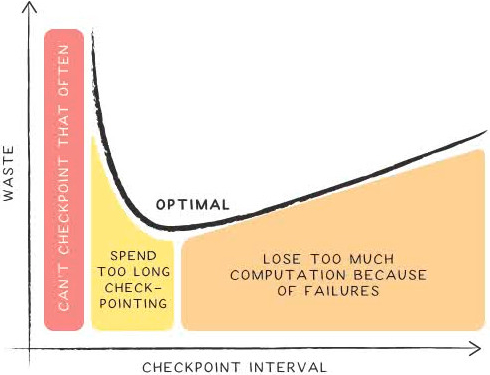
\includegraphics[width=\columnwidth]{resilience}
    \end{center}
  \end{column}
  \begin{column}{.4\linewidth}
    \small
    \textbf{First-order approximation [Young,Daly]:}\\
    Optimal period length:
    $$\blue{W^{\opt}} = \blue{\sqrt{2\mu C}}$$\\
    Corresponding overhead:
    $$\blue{H_{\text{opt}}} = \blue{\sqrt{\frac{2C}{\mu}}}$$
  \end{column}
\end{columns}

\end{frame}

\begin{frame}
  \frametitle{Hierarchical checkpointing}
  
\centerline{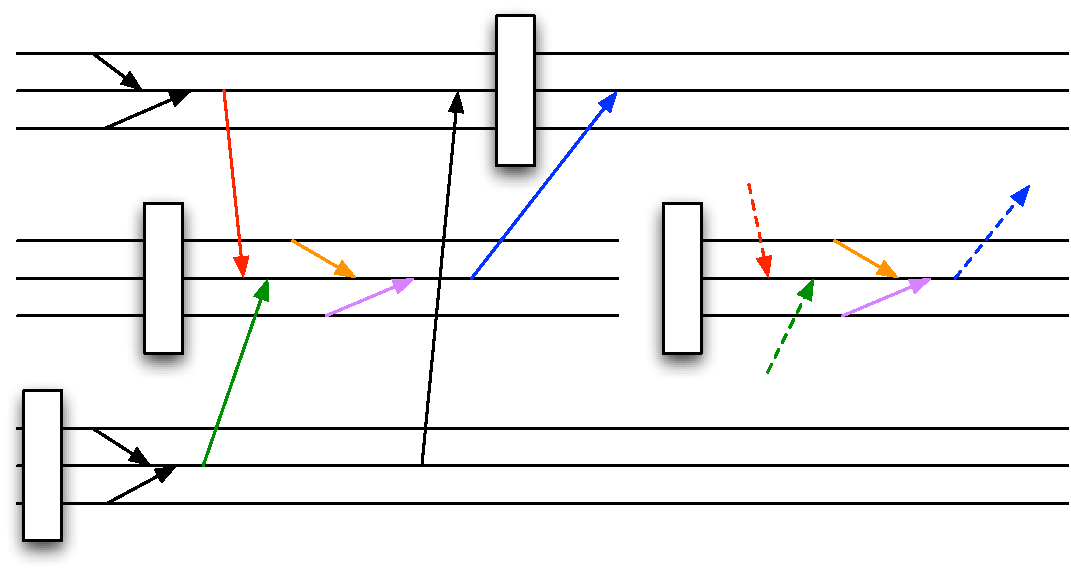
\includegraphics[width=.5\textwidth]{HierarFull.pdf}}

\vfill
  
\only<1>{\begin{itemize}
\item Non-coordinated protocols with Message Logging:
  \begin{itemize}
  \item Checkpoints are not coordinated
  \item Messages (and other nondeterministic events) are logged and replayed
  \end{itemize}
\item Hierarchical Protocols:
  \begin{itemize}
  \item Processors partitioned into $G$ groups of $q$ processors each
  \item Coordinated checkpointing inside each group, noncoordinated between groups
  \end{itemize}
\end{itemize}}
\only<2>{
  \begin{itemize}
  \item How to group processes:
    \begin{itemize}
    \item Per physical resources (high probability of simultaneous failure)
    \item Per communication group (high frequency of intra-group messages)
    \end{itemize}
  \item Expected advantages:
    \begin{itemize}
    \item[\smiley] no synchronization overheads 
    \item[\smiley] checkpoints are staggered
    \item[\smiley] only failed processes need to restart
    \end{itemize}
  \end{itemize}
}

\end{frame}

%% \begin{frame}
%%   \frametitle{Hierarchical Checkpointing: Failure during computing phase}

%%   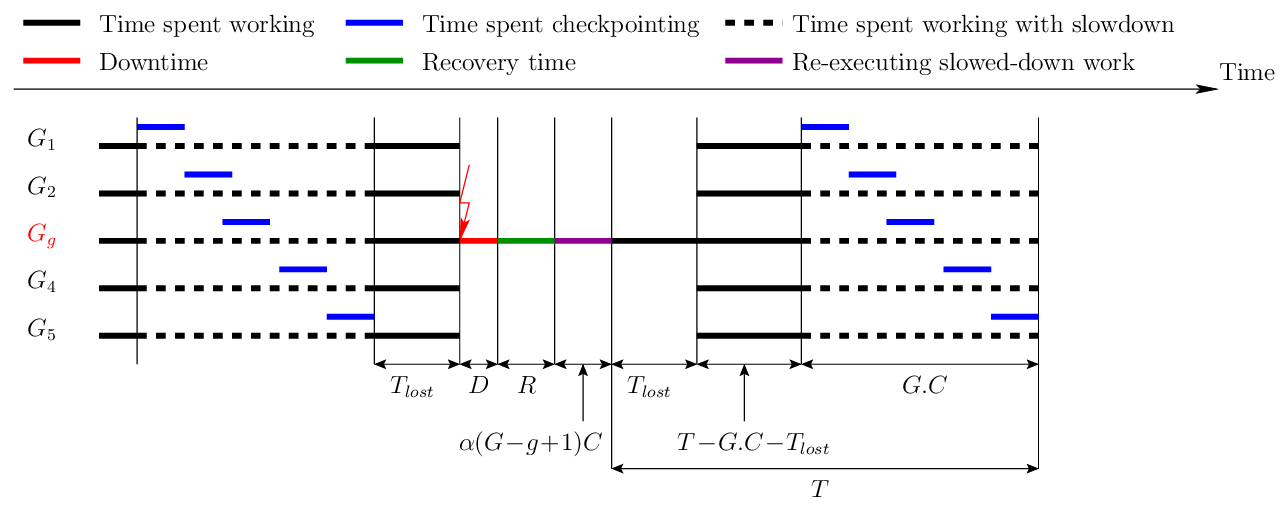
\includegraphics{hierarchical_failure_comp.png}

%%   \Overhead: $T_{lost}+\alpha(G-g+1)C$\\
%%   Expectation: $T_{lost}= \frac{1}{2}(T-G.C)$\\
%%   Approximated \Overhead: $\frac{T-G.C}{2}+\alpha(G-g+1)C$
  
%% \end{frame}

%% \begin{frame}
%%   \frametitle{Failure during checkpoint phase: Failure before checkpoint}

%%   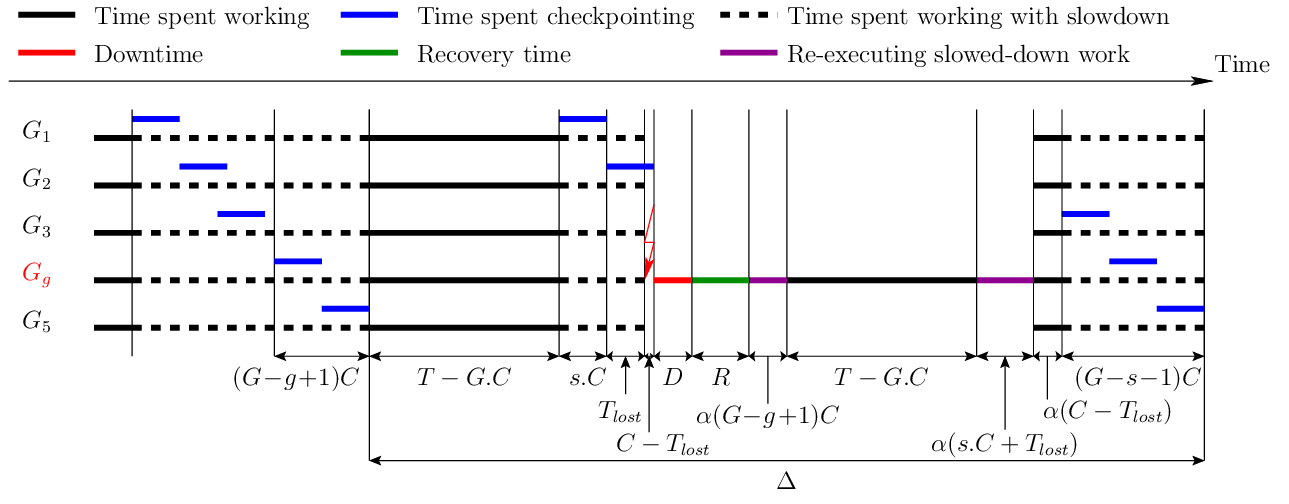
\includegraphics{hierarchical_failure_before_ckpt.png}

%%   Average \Overhead~for group $g$ (for $2 \leq g \leq G$):
%%     \begin{multline*}
%%       \frac{1}{g-1}\sum_{s=0}^{g-2} \left(T +
%%         ((\alpha-1)G+\alpha(-g+s+2)).C(q)\right) + D(q) + R(q)\\
%%       = T + D(q)+R(q)+\left((\alpha-1)G-\alpha\frac{g-2}{2}\right).C(q)
%%     \end{multline*}
  
%% \end{frame}

%% \begin{frame}
%%   \frametitle{Failure during checkpoint phase: Failure during checkpoint}

%%   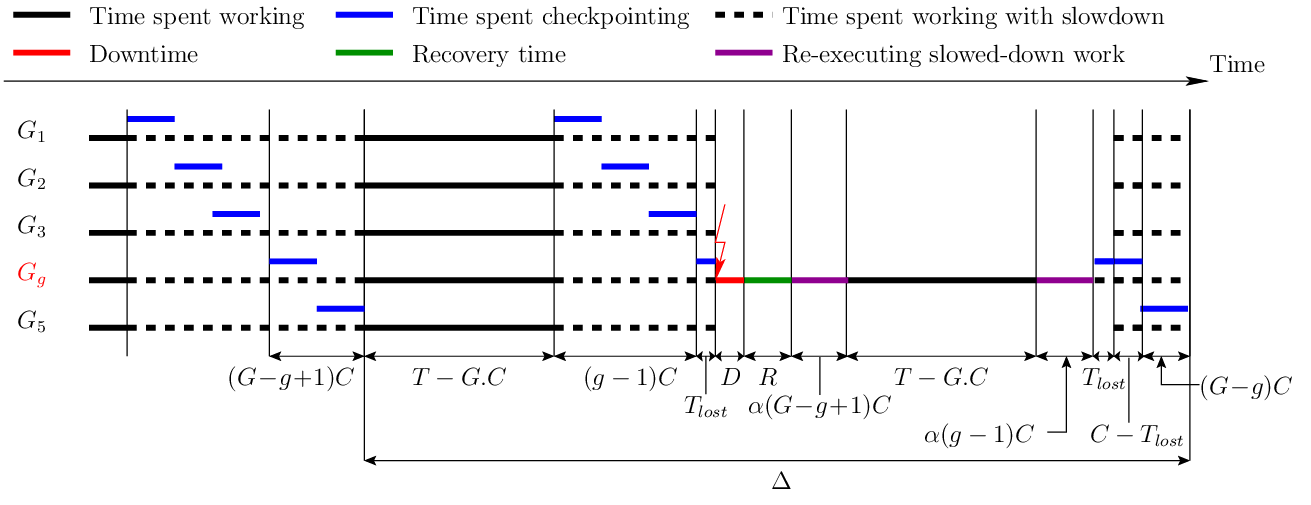
\includegraphics{hierarchical_failure_during_ckpt.png}

%%   \Overhead = $T+(\alpha-1)G.C + T_{lost}$
  
%%   Expectation: $T_{lost} = \frac{C}{2}$

%%   Approximated \Overhead  $$T+(\alpha-1)G.C(q)+\frac{C(q)}{2}$$
  
%% \end{frame}

%% \begin{frame}
%%   \frametitle{Failure during checkpoint phase: Failure after checkpoint}

%%   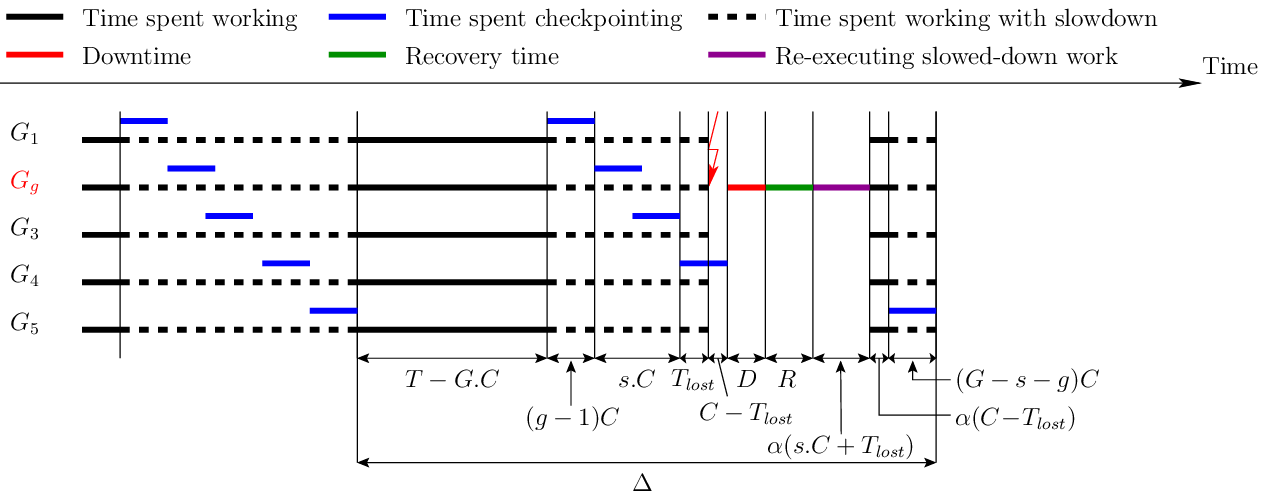
\includegraphics{hierarchical_failure_after_ckpt.png}

%%   \Overhead = $ \alpha(s+1)C$

%%   Average \Overhead~for group $g$ (for $1 \leq g \leq G-1$): 
%%   \begin{multline*}
%%     \frac{1}{G-g}\sum_{s=1}^{G-g}\left(\alpha(s+1)C(q)\right)= \alpha\frac{G-g+3}{2}C(q)
%%   \end{multline*}
  
%% \end{frame}

%% \begin{frame}
%%   \frametitle{Average waste for failures during checkpointing
%%     phase}
  
%%   Average \Overhead\ when the failing-group $g$ fails

%%   Overall average \Overhead: $\ockpt = $\\[-5mm]
%%   \begin{multline*}
%%     \frac{1}{G} ( (g\!-\!1) . \obckpt +
%%       1.  \odckpt\\ + (G\!-\!g) . \oackpt)
%%   \end{multline*}
%%   \vfill
%%     Average over all groups:
%%     \begin{multline*}
%%       \avgockpt =\\ \frac{G+1}{2G}T + \frac{\alpha
%%         C(q)(G+3)}{2}+\frac{C(q)(1-2\alpha)}{2G} -\frac{C(q)(G+1)}{2}
%%     \end{multline*}
%% \end{frame}

%% \begin{frame}
%%   \frametitle{Total waste}
  
%%   $$
%%   \begin{array}{l}
%%     \displaystyle \Waste[FF] =  \frac{T-\Work}{T} \text{ with } \Work = T - (1-\alpha) G C(q)\\
%%     \displaystyle \Waste[fail] = \frac{1}{\muplatform} \bigg( \dgroup + \rgroup + \Overhead \bigg) \text{ with } \\[3mm]
%%     \displaystyle \Overhead =   \frac{\T\!-\!\ngroups\cgroup}{\T} \ocomp +  \frac{\ngroups\cgroup}{\T} \ockpt \\[5mm]
%%       \displaystyle \Waste = \Waste[FF] + \Waste[fail] - \Waste[FF] \Waste[fail]
%%  \end{array}
%%  $$ 
%% \end{frame}

%% \begin{frame}
%%   \frametitle{Accounting for message logging: Impact on work}

%%  \begin{itemize}
%%   \item \frownie Logging messages slows down execution:\\
%%   $\Rightarrow$ $\Work$ becomes $\red{\lambda} \Work$, where $0 < \lambda <1$\\
%%   Typical value: $ \lambda \sim 0.98$

%%   \item \smiley Re-execution after a failure is faster:\\
%%   $\Rightarrow$ $\Overhead$ becomes $\frac{\Overhead}{\red{\rho}}$, where $\rho \in[1..2]$\\
%%    Typical value: $ \rho \sim 1.5$
  
%%   \end{itemize}

%% \vfill
%% $$\Waste[FF] = \frac{\T - \red{\lambda} \Work}{\T}$$
%% $$\Waste[fail] = \frac{1}{\muplatform} \bigg( \dgroup + \rgroup + 
%% \frac{\Overhead}{\red{\rho}} \bigg) $$
%% \end{frame}


%% \begin{frame}
%%   \frametitle{Accounting for message logging: Impact on checkpoint size}

%%  \begin{itemize}
%%  \item Inter-groups messages logged continuously
%%  \item  Checkpoint size increases with amount of work executed before a checkpoint
%%  \item $\cgroupbase$: Checkpoint size of a group without message logging
%% $$
%% \cgroup = \cgroupbase (1 + \amountlog \Work) \Leftrightarrow \color{red}{\amountlog = \frac{\cgroup - \cgroupbase}{\cgroupbase \Work}}
%% $$
%% %\begin{overlayarea}{\linewidth}{2cm}{
%% $$\Work = \lambda (\T - (1-\workduringckpt)\ngroups\cgroup)$$
%% $$\cgroup = \frac{ \cgroupbase (1 + \amountlog \lambda \T)}{1+ \ngroups \cgroupbase \amountlog \lambda (1-\workduringckpt)}$$

%% %\end{overlayarea}
%% %% \item
%% %% Constraint $ \ngroups \cgroup \leq \T$ translates into 
%% %% $$
%% %% \ngroups \cgroupbase \amountlog \lambda \workduringckpt \leq 1 \text{ and } \T \geq \frac{\ngroups \cgroupbase }{1- \ngroups \cgroupbase \amountlog \lambda \workduringckpt} $$

%%  \end{itemize}

%%  \vfill
%%  Minimize $\Waste$ subject to:
%%   \begin{itemize}
%%   \item $G C(q) \leq T$ (by construction)
%%   \item Gets complicated! Use computer algebra software \frownie
%%   \end{itemize}
%% \end{frame}

\begin{frame}
  \frametitle{Modeling Hierarchical Protocols}

  \begin{center}
    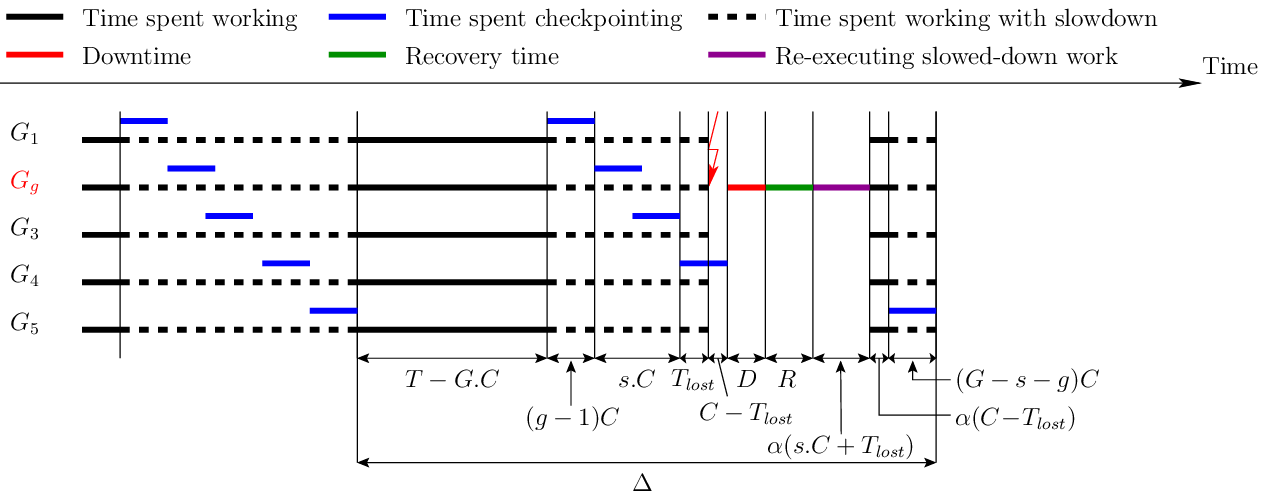
\includegraphics[scale=0.7]{hierarchical_failure_after_ckpt.png}
  \end{center}

  Modeling the hierarchical protocol is challenging compared to the coordinated one
  
  \begin{columns}
    \begin{column}{.49\textwidth}
      \begin{itemize}
      \item Which group is subject to failure
      \item Failure between two checkpoint waves
      \item Failure within a wave
        \begin{itemize}
        \item but before the group checkpoint
        \item during the group checkpoint
        \item after the group checkpoint
        \end{itemize}
      \end{itemize}
    \end{column}\begin{column}{.49\textwidth}
      \begin{itemize}
      \item Message logging impacts:
        \begin{itemize}
        \item Work speed (re-execution is slightly faster)
        \item Checkpoint size (and duration)
          \begin{itemize}
          \item Checkpoint size increases with amount of work executed before the checkpoint
          \end{itemize}
        \end{itemize}
      \end{itemize}
    \end{column}
  \end{columns}
  
\end{frame}

\begin{frame}
  \frametitle{Platforms: basic characteristics}
  
  \begin{center}\sffamily\scriptsize
    \resizebox{0.9\linewidth}{!}
    %\scalebox{0.85}
    {\hspace*{-1cm} \begin{tabular}{|c|c|c|c|c|c|c|c|}\hline
        Name 			& Number of     & Number of 			& Number of cores	& Memory  		& \multicolumn{2}{c|}{I/O Network Bandwidth (\bwio)} 	& I/O Bandwidth (\bwnode)\\
        &  cores     	& processors \nprocess  & per processor     & per processor & Read 		& Write 									& Read/Write per processor \\\hline
        Titan  			& 299,008       & 16,688  				& 16                & 32GB 			& 300GB/s 	& 300GB/s 									& 20GB/s \\\hline
        Exascale-Slim 	& 1,000,000,000 & 1,000,000 			& 1,000             & 64GB         	& 1TB/s     & 1TB/s     								& 200GB/s \\\hline
        Exascale-Fat	& 1,000,000,000 & 100,000 				& 10,000            & 640GB       	& 1TB/s     & 1TB/s     								& 400GB/s \\\hline
      \end{tabular}}
  \end{center}

\vfill

\begin{center}%\sffamily\scriptsize
\resizebox{0.7\linewidth}{!}
%\scalebox{0.85}
{\begin{tabular}{|c|c|c|c|c|c|c|}
\hline
Name 			& Scenario	& \ngroups (\cgroup) 	& \amountlog for  	& \amountlog for \\
          		&           & 					 	& \StenTwo 			&  \Matprod \\\hline
                                                    
          		& \CSCI     & 1 (2,048s) 			& / 				& /\\
Titan  			& \CSHI     & 136 (15s)   			& 0.0001098         & 0.0004280 \\ 
          		& \CSHP    	& 1,246 (1.6s) 			& 0.0002196  		& 0.0008561  \\\hline
                                        			                                        			
            	& \CSCI   	& 1 (1,000s/100s)		& / 				& /  \\
Exascale-Slim	& \CSHI 	& 1,000 (64s)   		& 0.0002599         & 0.001013      \\ 
         		& \CSHP 	& 200,0000 (0.32s) 		& 0.0005199  		& 0.002026   \\\hline
                                        			
         		& \CSCI   	& 1 (1,000s/100s)		& / 				& /  \\
Exascale-Fat	& \CSHI 	& 316 (217s)  			& 0.00008220        & 0.0003203 \\ 
         		& \CSHP 	& 33,3333 (1.92s)		& 0.00016440    	& 0.0006407 \\\hline
\end{tabular}}

$\alpha = 0.3$, $\lambda = 0.98$ and $\rho = 1.5$
\end{center}

\end{frame}


\begin{frame}
\frametitle{Waste for Titan}
\vfill
\begin{tabular}{p{.3\textwidth}p{.3\textwidth}p{.3\textwidth}}
Stencil 2D & Matrix product & Stencil 3D\\
   \hspace{1cm} 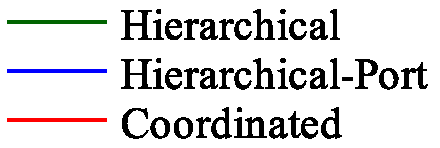
\includegraphics[width=0.3\linewidth]{3courbes.pdf} &
  \hspace{1.3cm} 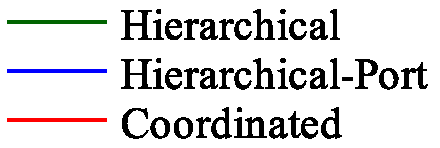
\includegraphics[width=0.3\linewidth]{3courbes.pdf}&
 \hspace{1.5cm}  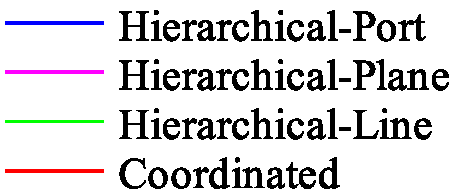
\includegraphics[width=0.2\linewidth]{4courbes.pdf} \\
  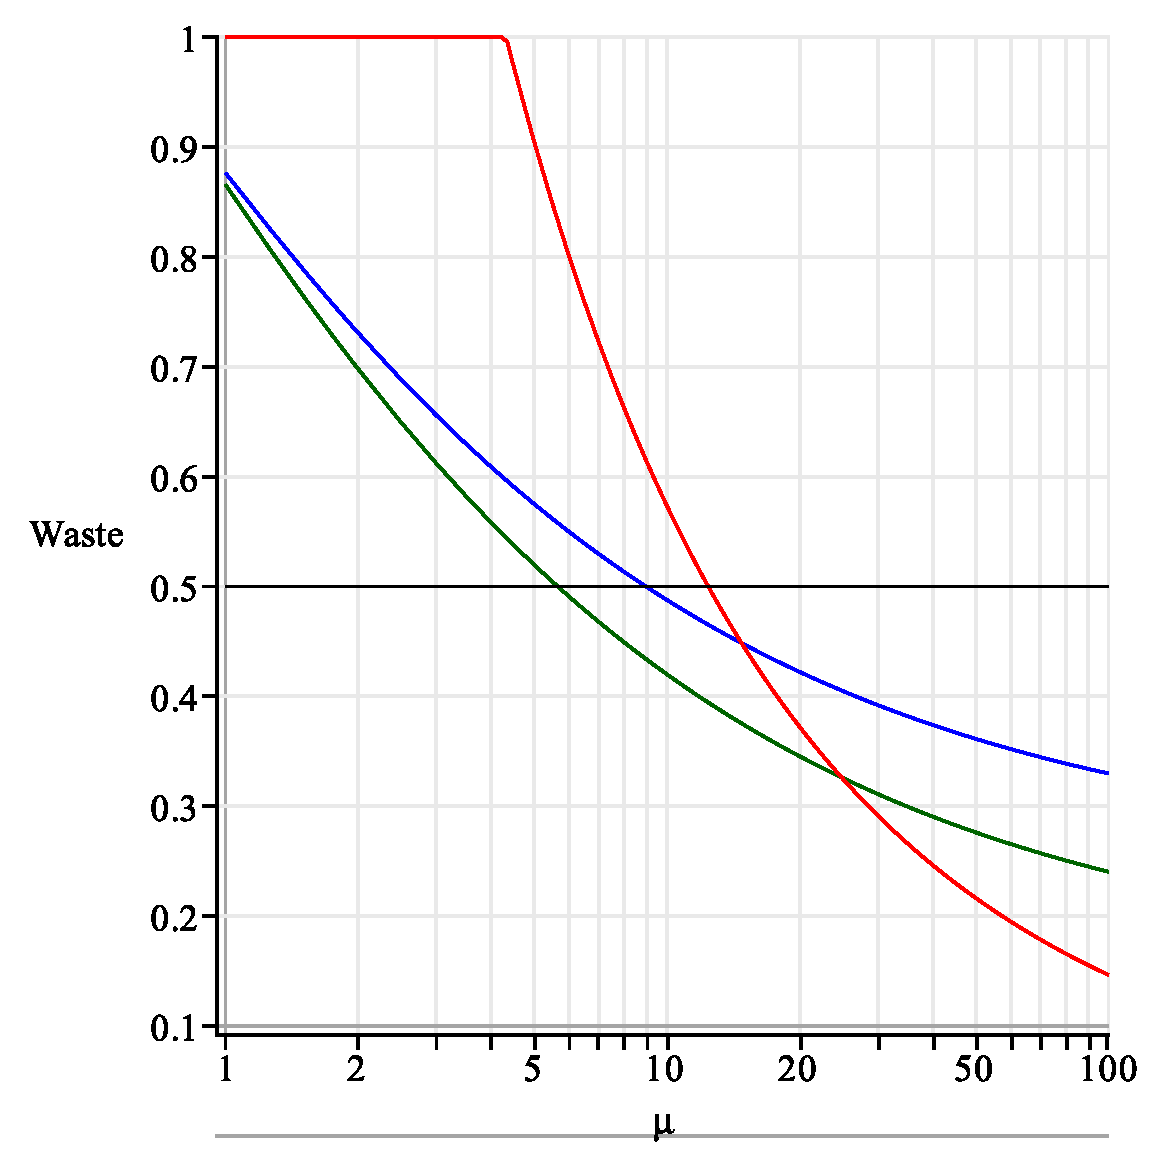
\includegraphics[width=0.3\textwidth,height=0.32\textheight,viewport=70 35 555 555,clip]{TitanWasteStenc.pdf} &
  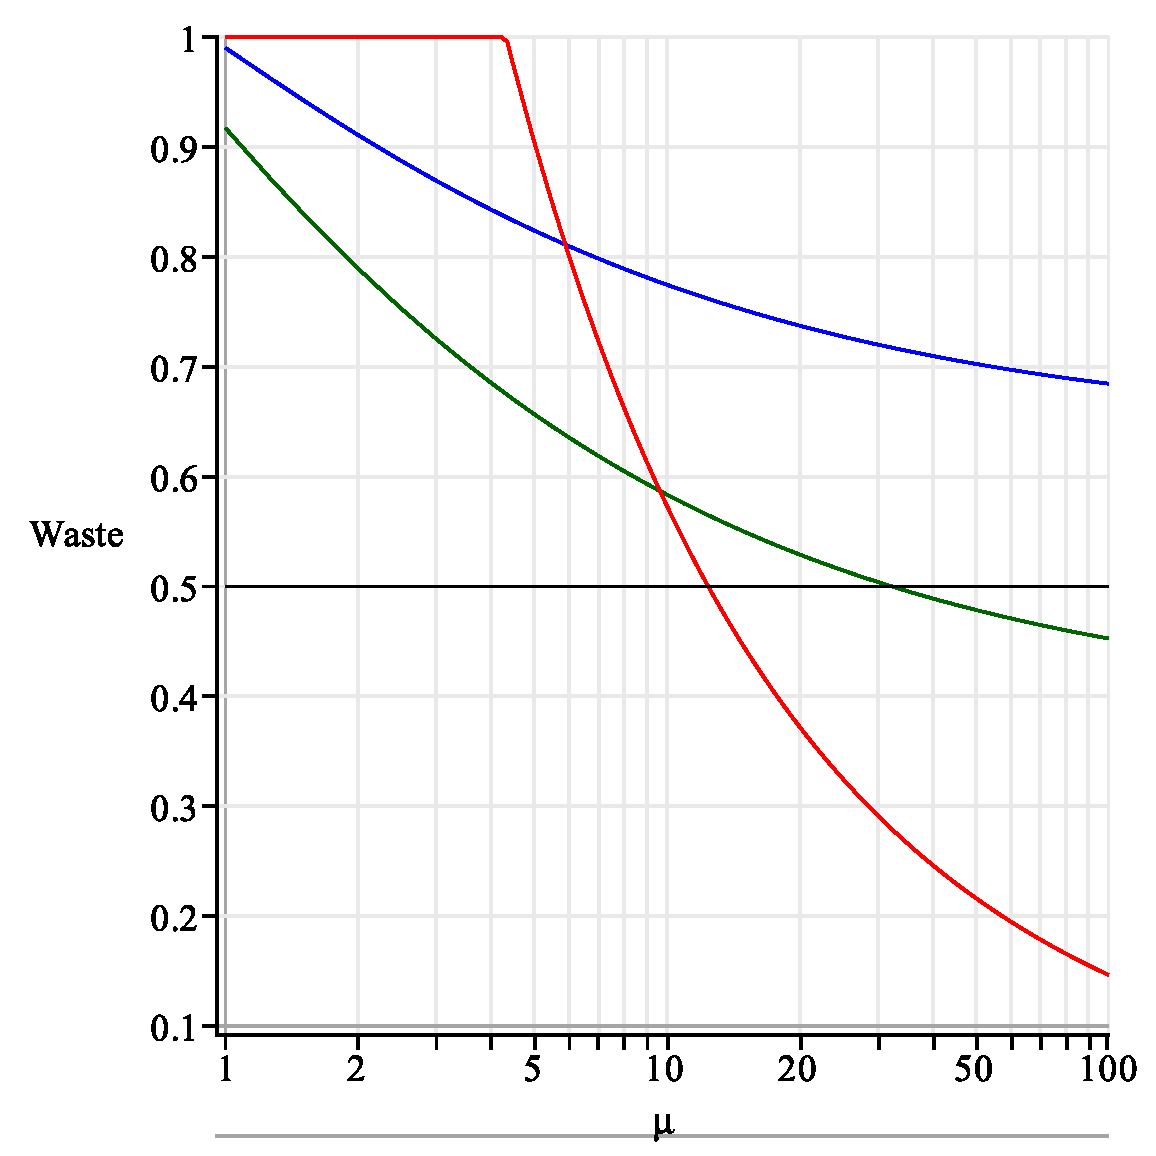
\includegraphics[width=0.3\textwidth,height=0.32\textheight,viewport=70 35 555 555,clip]{TitanWasteMat.pdf} &
  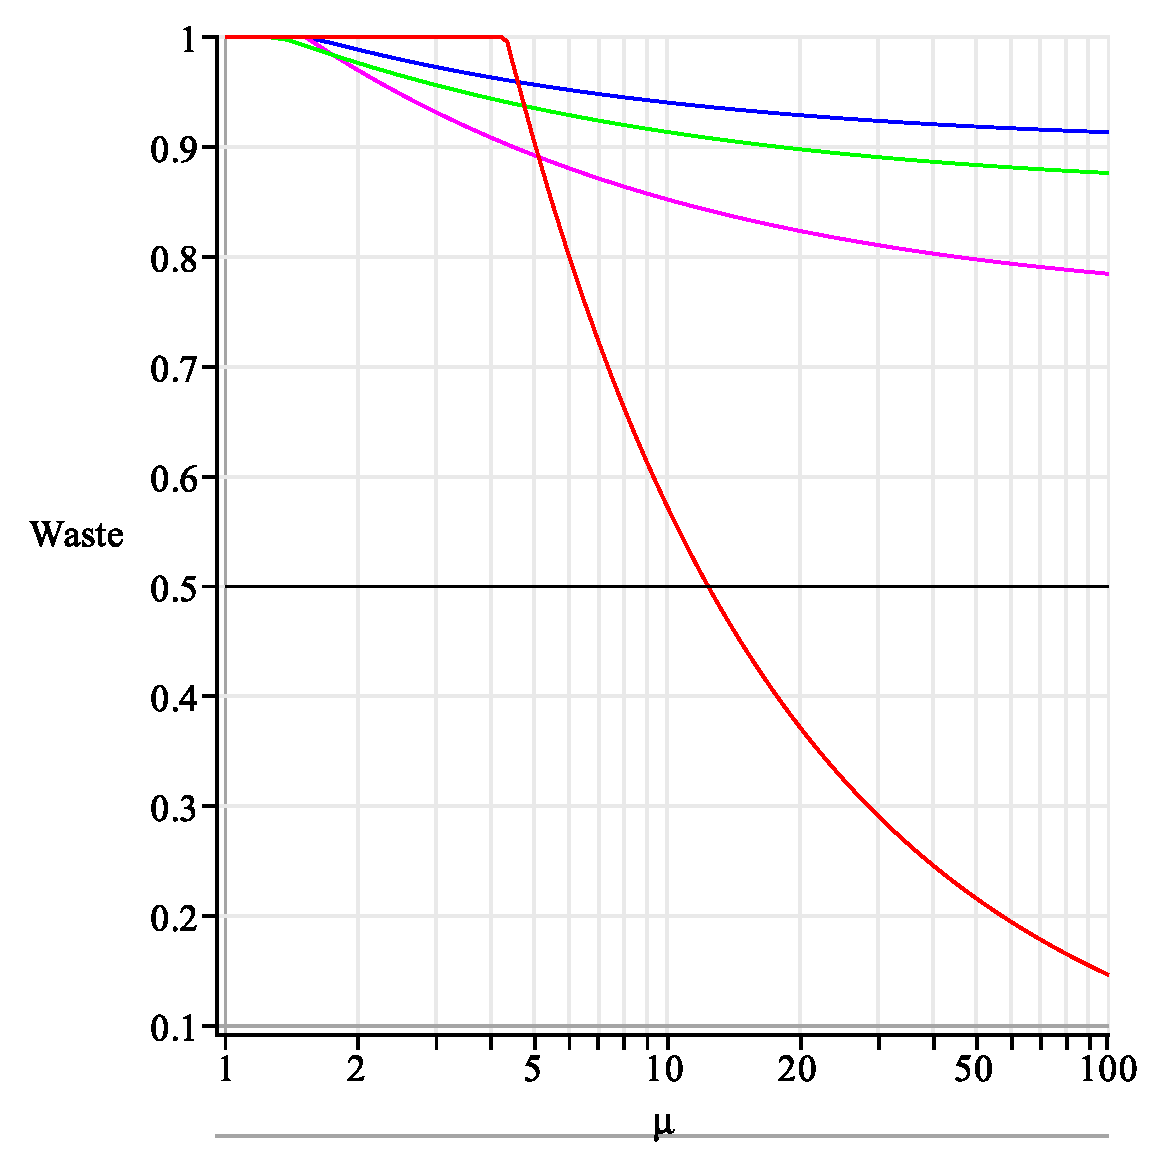
\includegraphics[width=0.3\textwidth,height=0.32\textheight,viewport=70 35 555 555,clip]{TitanWasteStenc3D.pdf} 
 \end{tabular}
 ~\\
\centerline{Waste as a function of processor MTBF $\mu_{ind}$}
\end{frame}


\begin{frame}
\frametitle{Waste for Prospective Exascale Platforms with $C=1,000$}
\vfill
\begin{tabular}{cp{.3\textwidth}p{.3\textwidth}p{.3\textwidth}}
& Stencil 2D & Matrix product & Stencil 3D\\
  & \hspace{1cm} 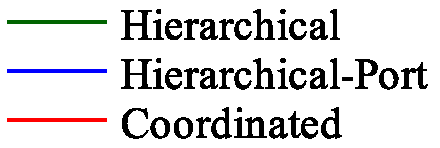
\includegraphics[width=0.3\linewidth]{3courbes.pdf} &
  \hspace{1.5cm} 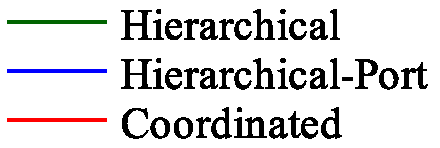
\includegraphics[width=0.3\linewidth]{3courbes.pdf}&
 \hspace{2cm}  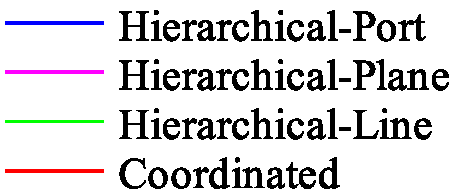
\includegraphics[width=0.2\linewidth]{4courbes.pdf} \\
 \rotatebox{90}{\hspace{.5cm}Exascale-Slim} &
  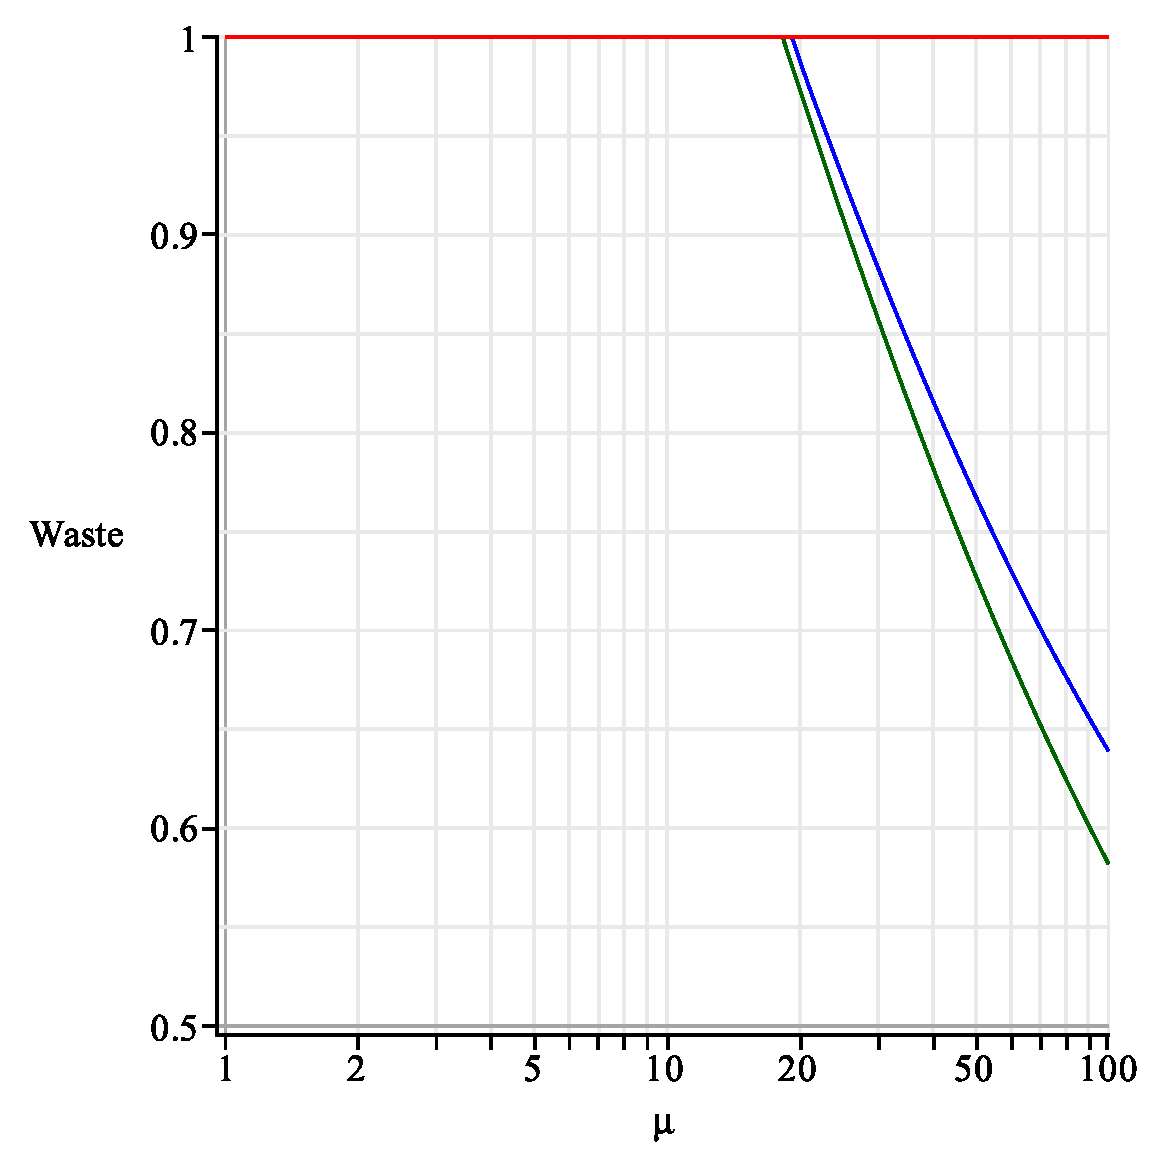
\includegraphics[width=0.3\textwidth,height=0.32\textheight,viewport=70 35 555 555,clip]{SlimWasteStenc1000.pdf} &
  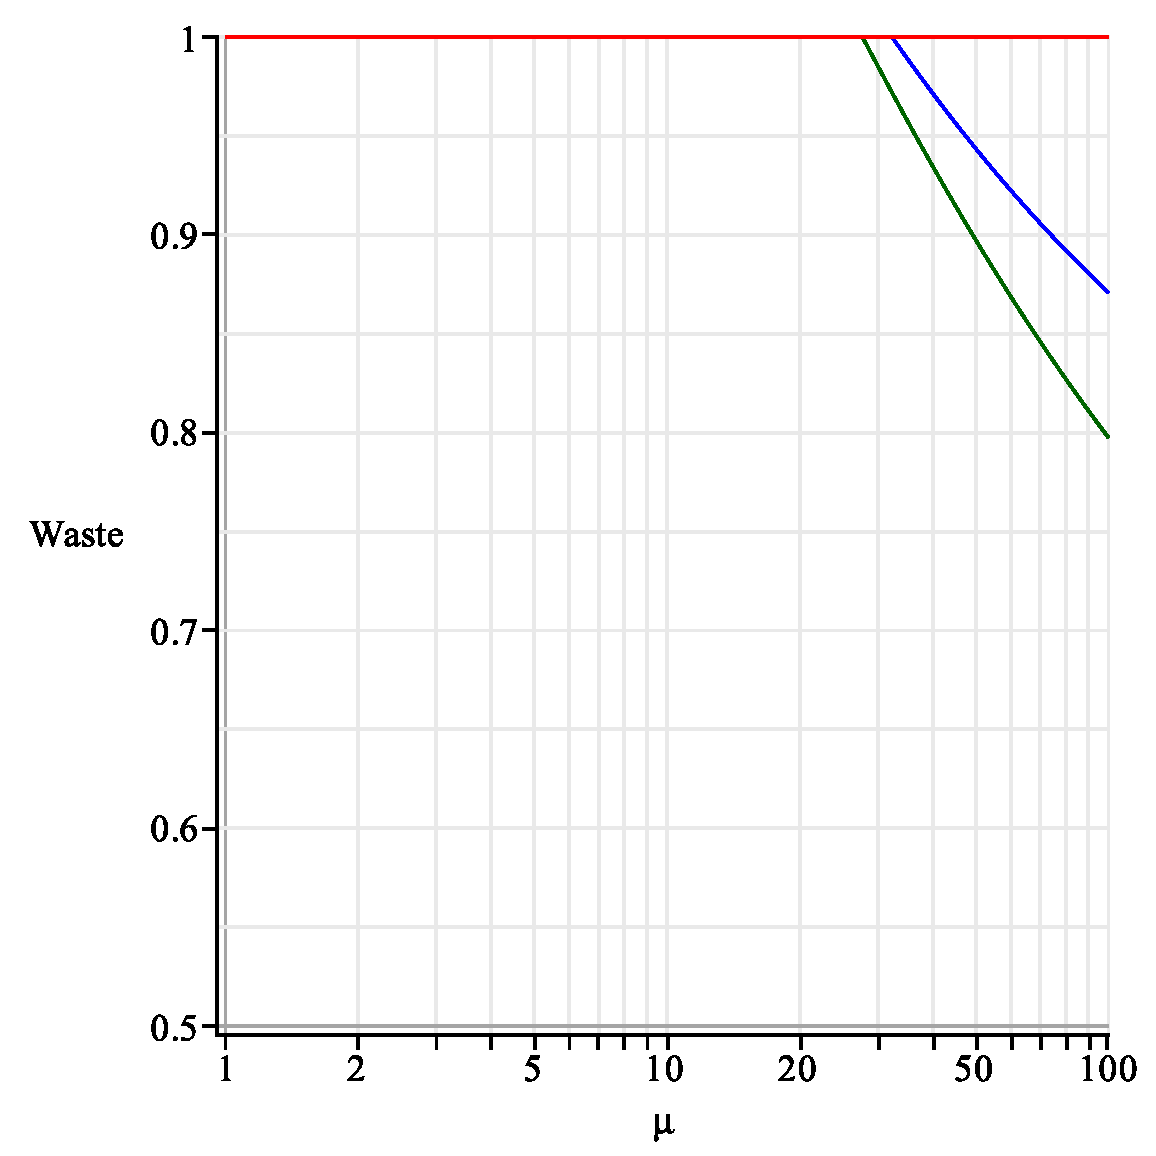
\includegraphics[width=0.3\textwidth,height=0.32\textheight,viewport=70 35 555 555,clip]{SlimWasteMat1000.pdf} &
  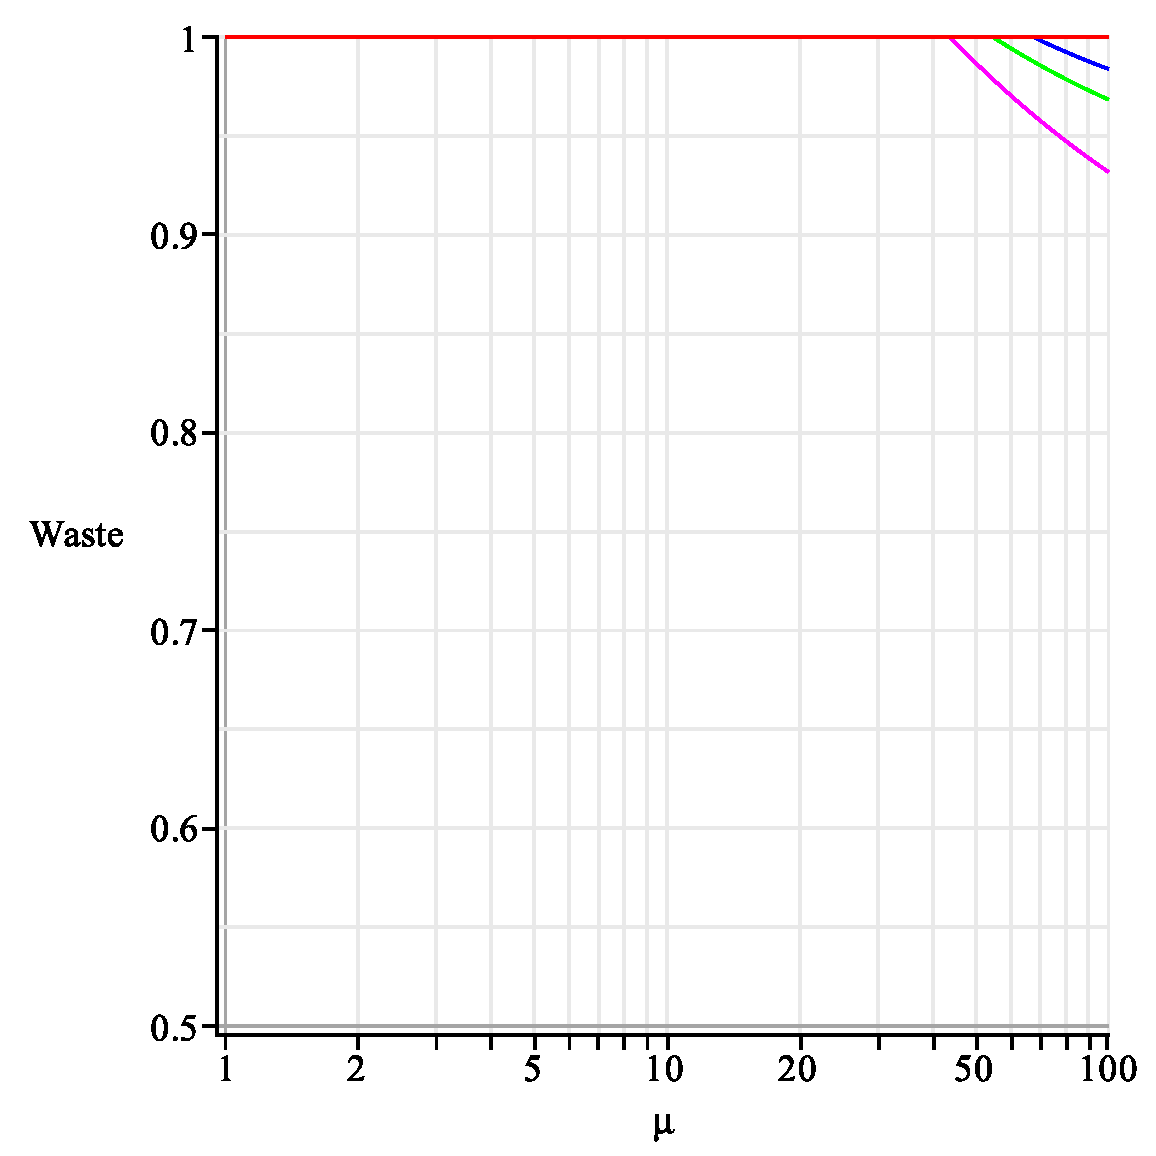
\includegraphics[width=0.3\textwidth,height=0.32\textheight,viewport=70 35 555 555,clip]{SlimWasteStenc3D1000.pdf} \\
   \rotatebox{90}{\hspace{.5cm}Exascale-Fat} &
    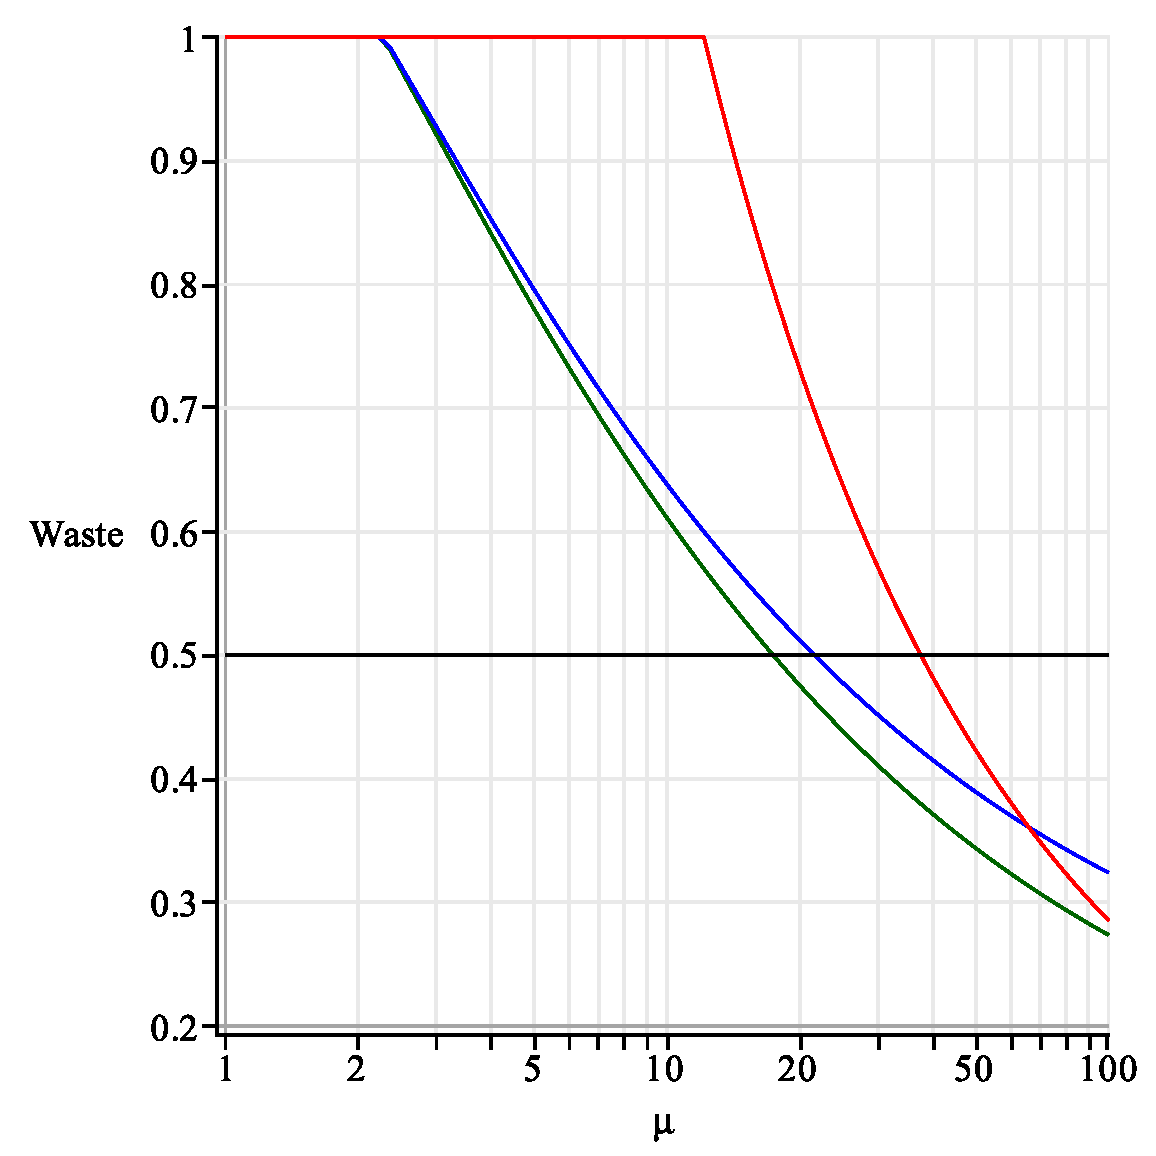
\includegraphics[width=0.3\textwidth,height=0.32\textheight,viewport=70 35 555 555,clip]{FatWasteStenc1000.pdf} &
  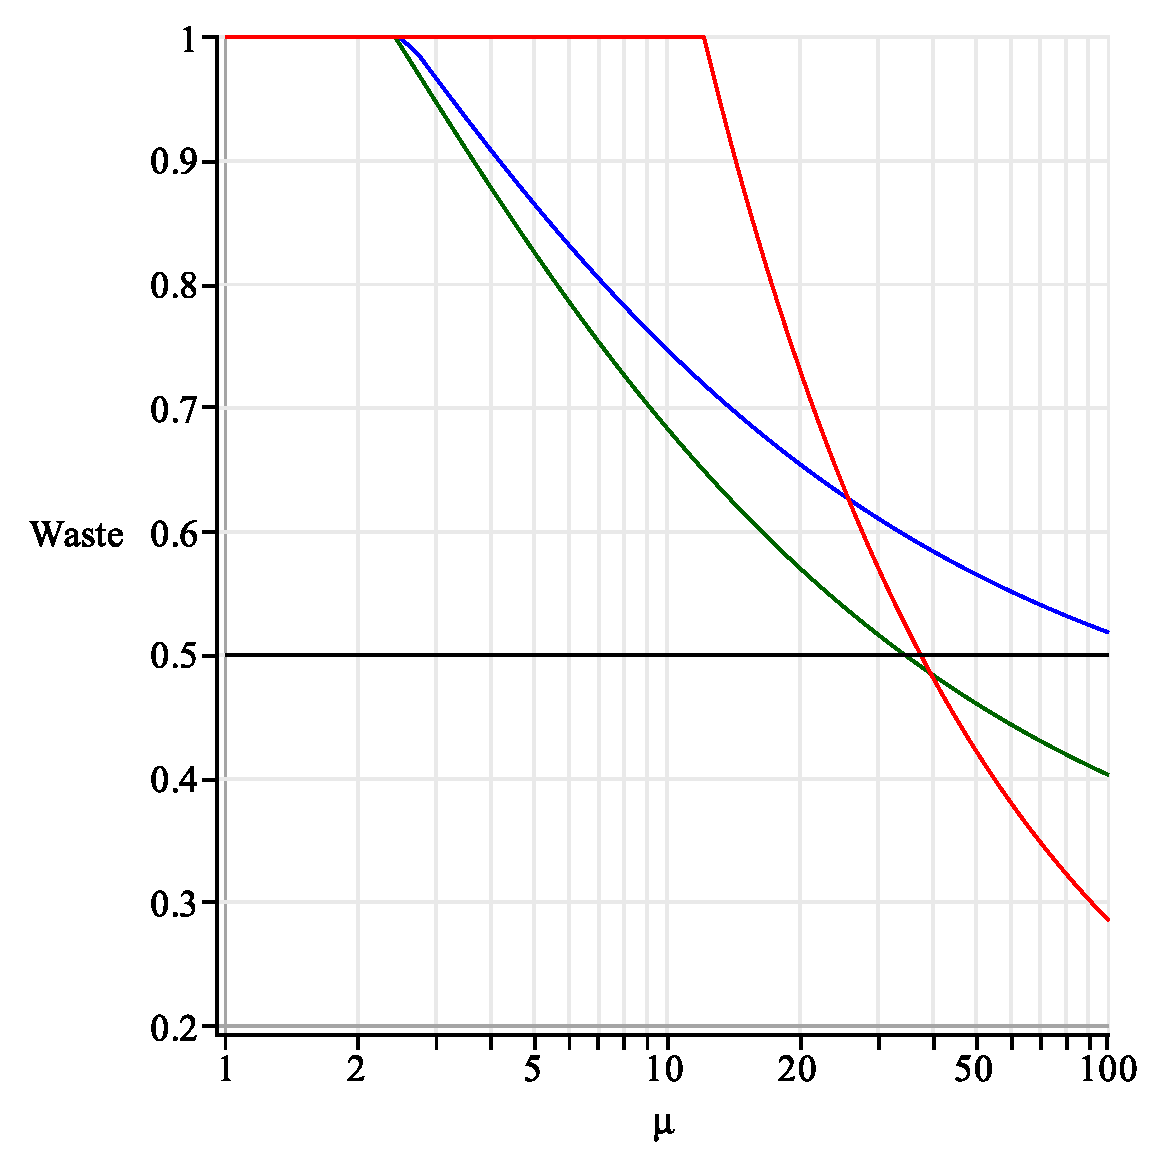
\includegraphics[width=0.3\textwidth,height=0.32\textheight,viewport=70 35 555 555,clip]{FatWasteMat1000.pdf} &
  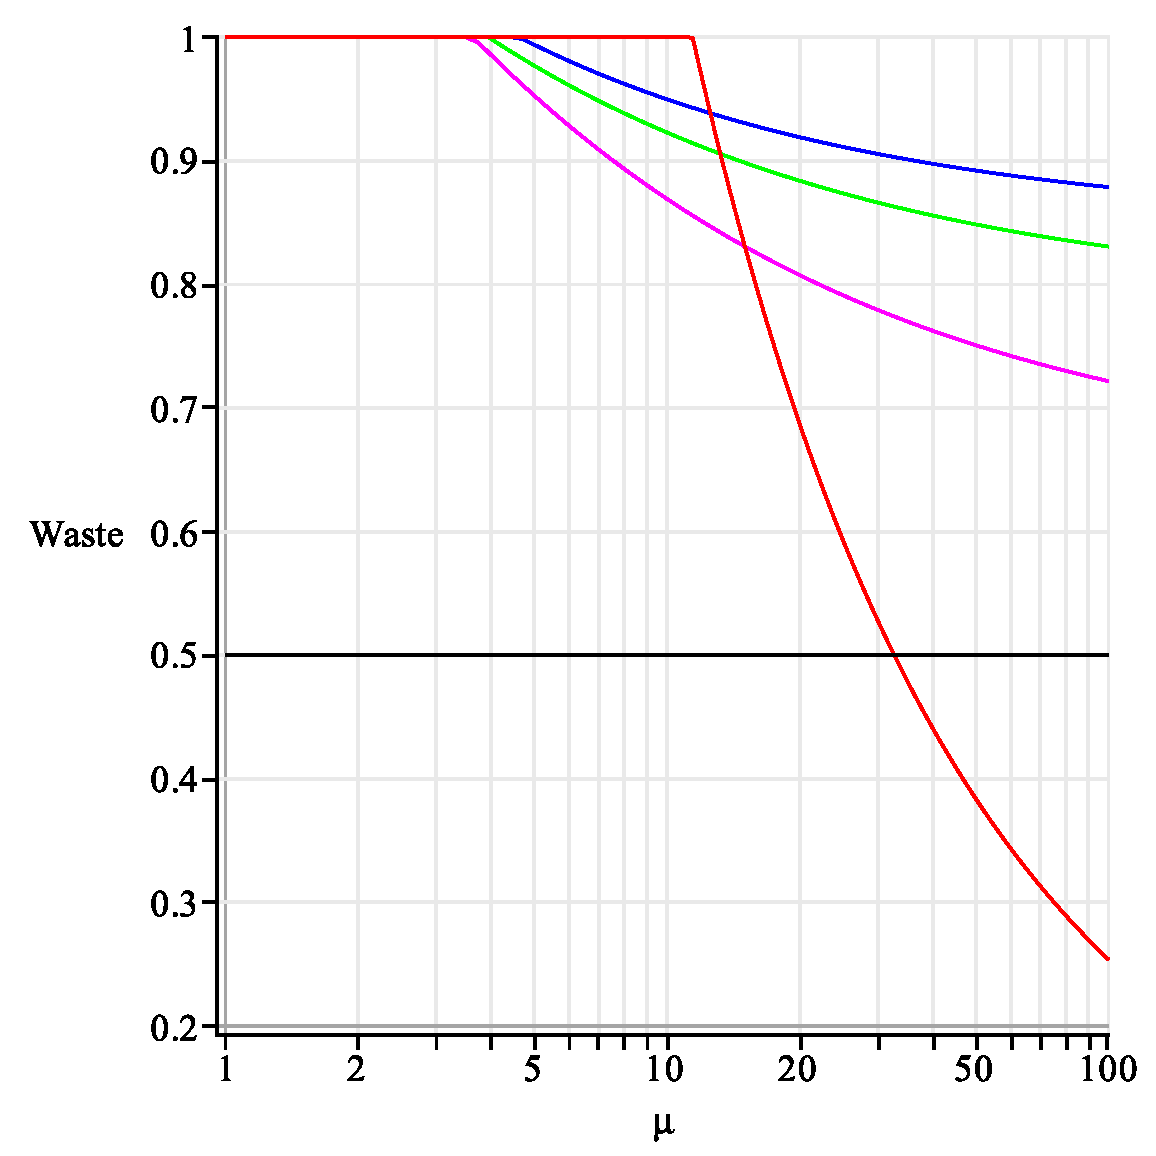
\includegraphics[width=0.3\textwidth,height=0.32\textheight,viewport=70 35 555 555,clip]{FatWasteStenc3D1000.pdf} \\
 \end{tabular}
 ~\\
\centerline{Waste as a function of processor MTBF $\mu_{ind}$, $C=1,000$}
\end{frame}

\begin{frame}
\frametitle{Waste for Prospective Exascale Platforms with $C=100$}
\vfill
\begin{tabular}{cp{.3\textwidth}p{.3\textwidth}p{.3\textwidth}}
& Stencil 2D & Matrix product & Stencil 3D\\
  & \hspace{1cm} 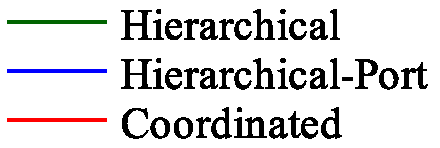
\includegraphics[width=0.3\linewidth]{3courbes.pdf} &
  \hspace{1.5cm} 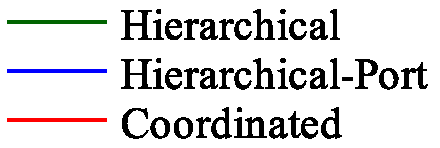
\includegraphics[width=0.3\linewidth]{3courbes.pdf}&
 \hspace{2cm}  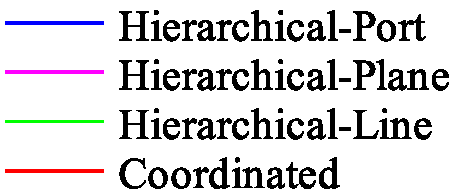
\includegraphics[width=0.2\linewidth]{4courbes.pdf} \\
 \rotatebox{90}{\hspace{.5cm}Exascale-Slim} &
  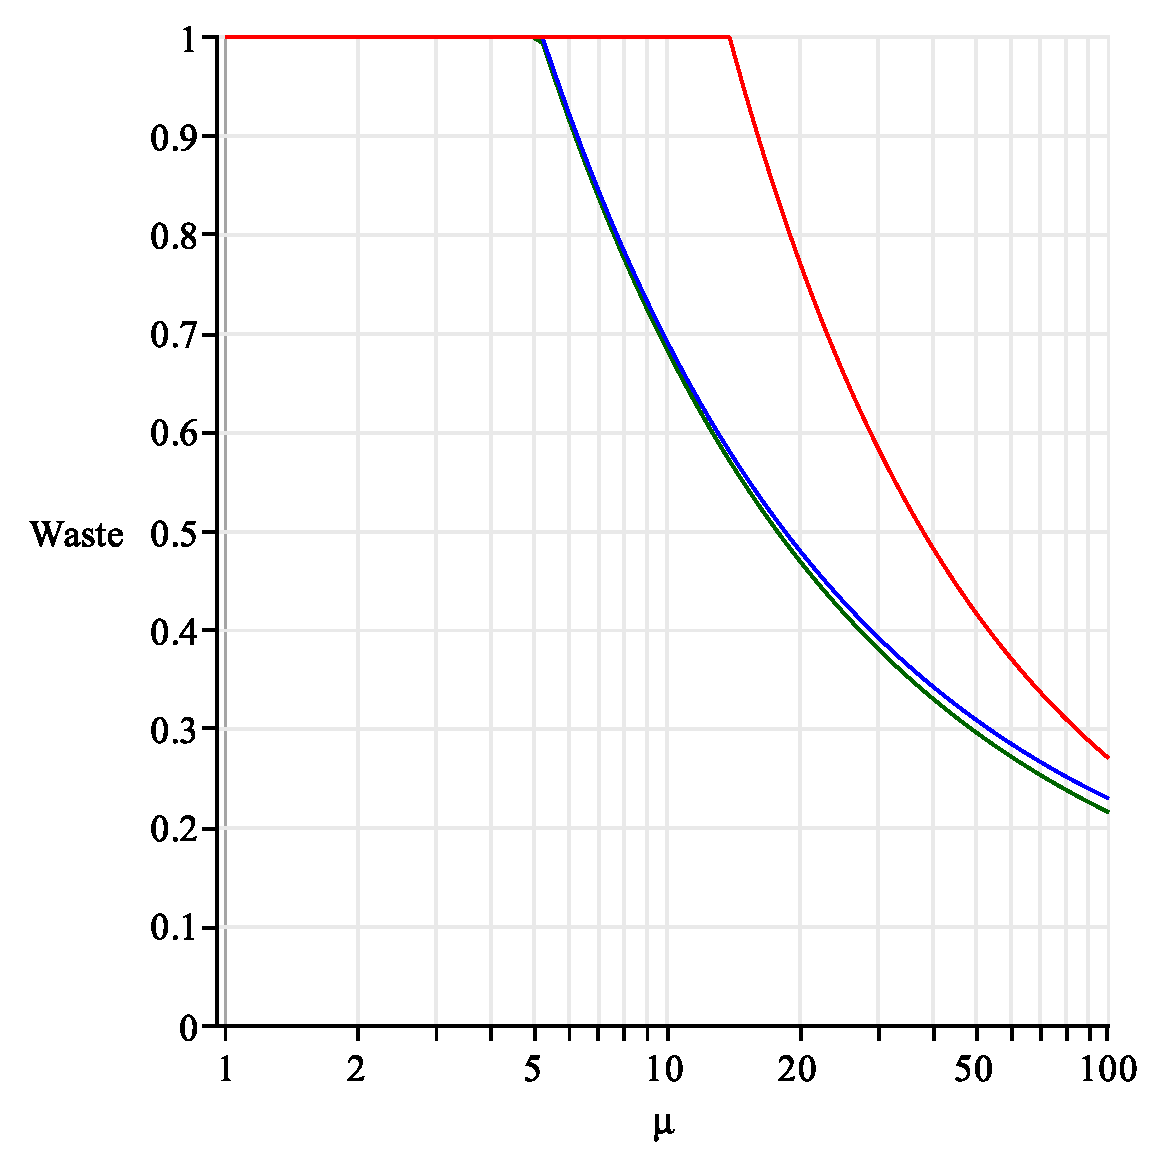
\includegraphics[width=0.3\textwidth,height=0.32\textheight,viewport=70 35 555 555,clip]{SlimWasteStenc100.pdf} &
  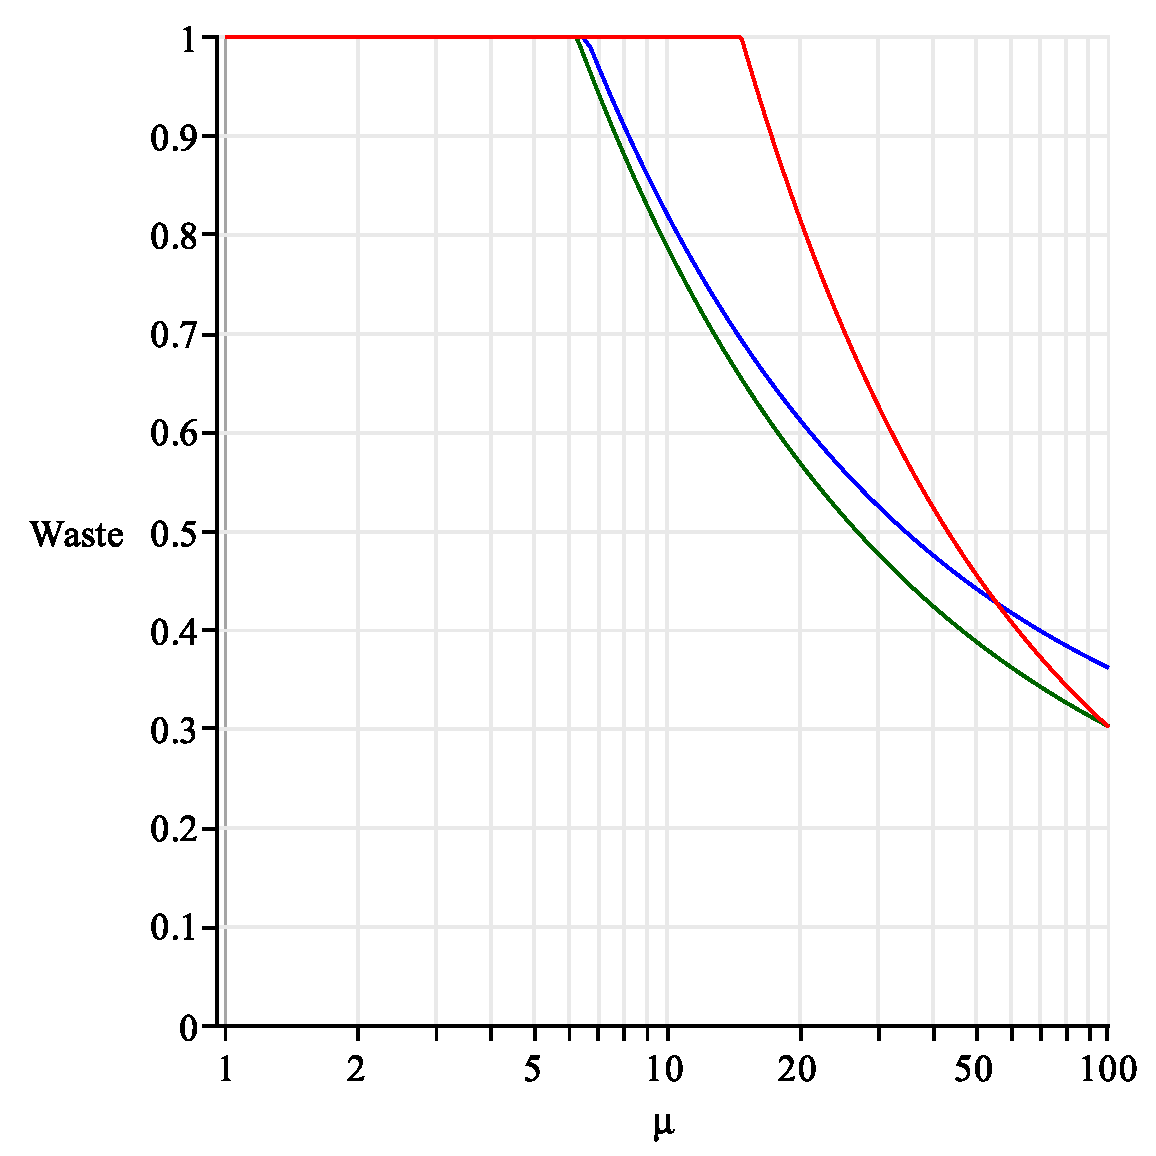
\includegraphics[width=0.3\textwidth,height=0.32\textheight,viewport=70 35 555 555,clip]{SlimWasteMat100.pdf} &
  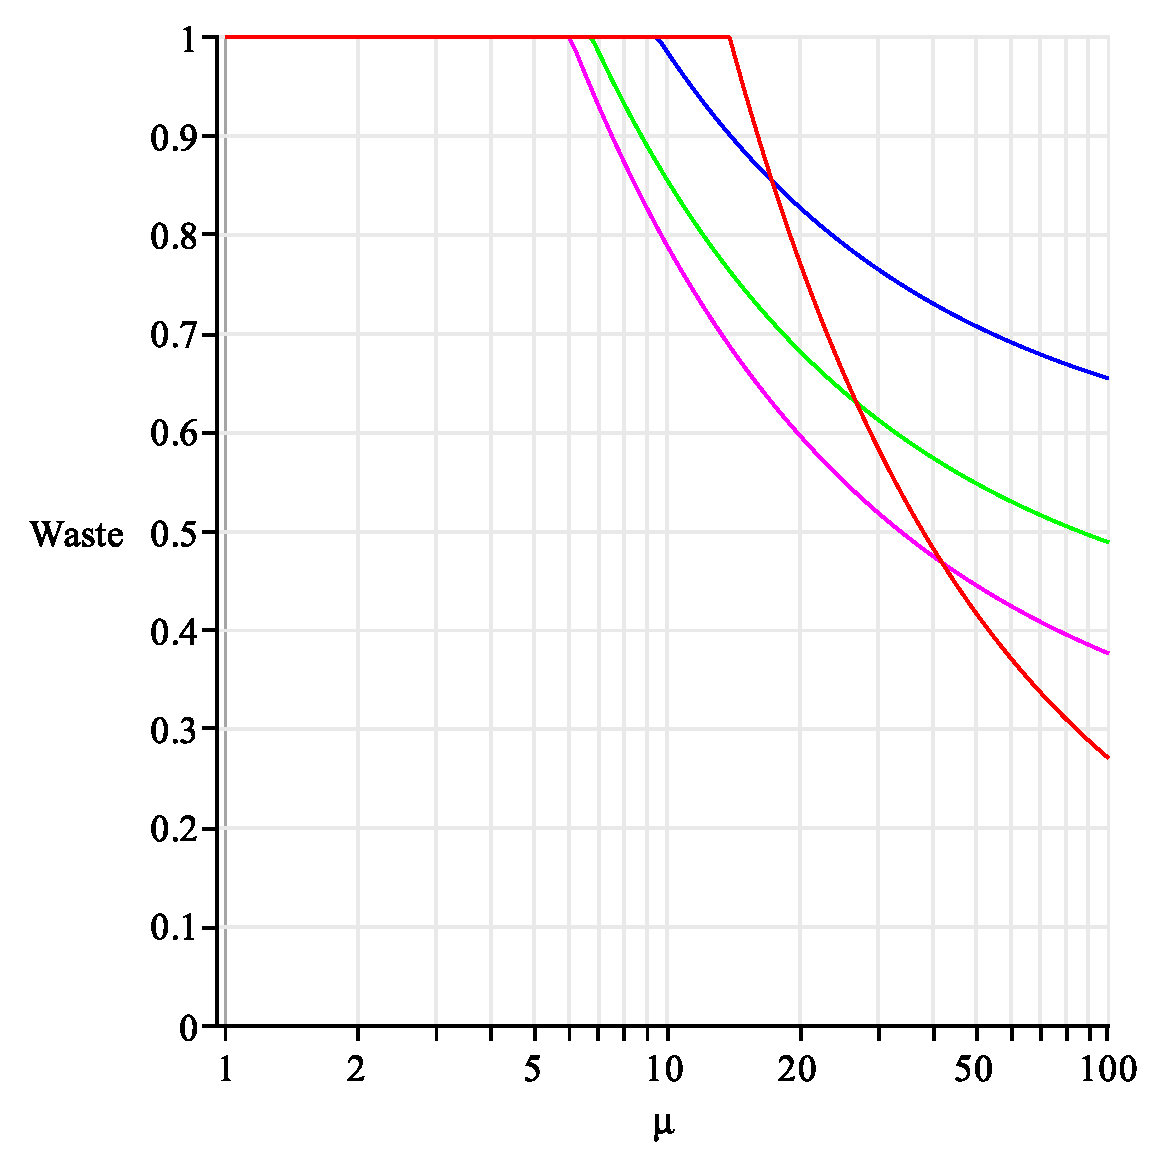
\includegraphics[width=0.3\textwidth,height=0.32\textheight,viewport=70 35 555 555,clip]{SlimWasteStenc3D100.pdf} \\
   \rotatebox{90}{\hspace{.5cm}Exascale-Fat} &
    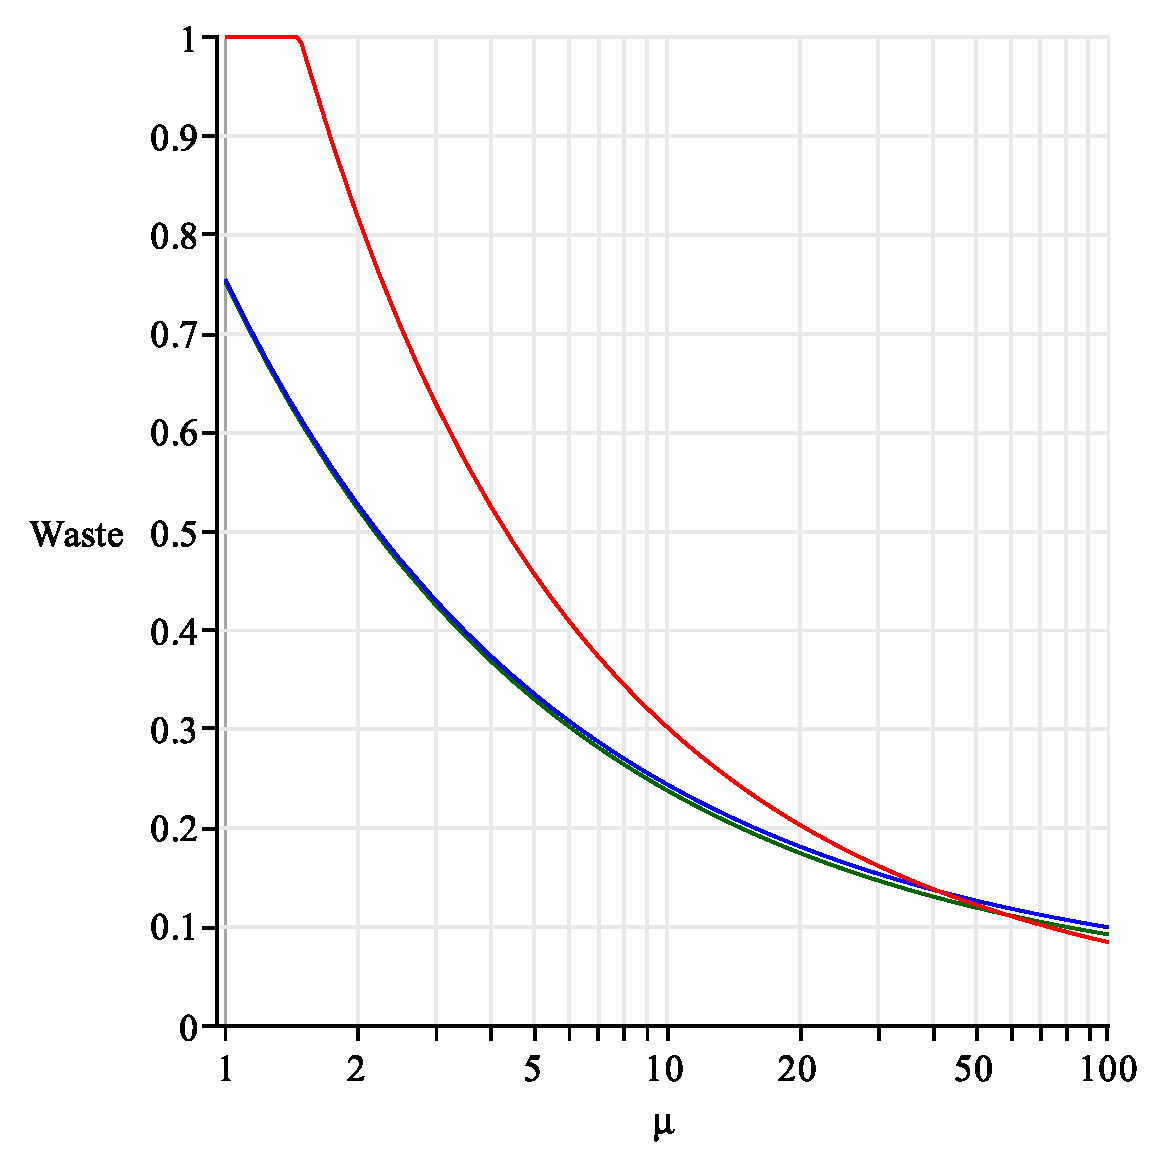
\includegraphics[width=0.3\textwidth,height=0.32\textheight,viewport=70 35 555 555,clip]{FatWasteStenc100.pdf} &
  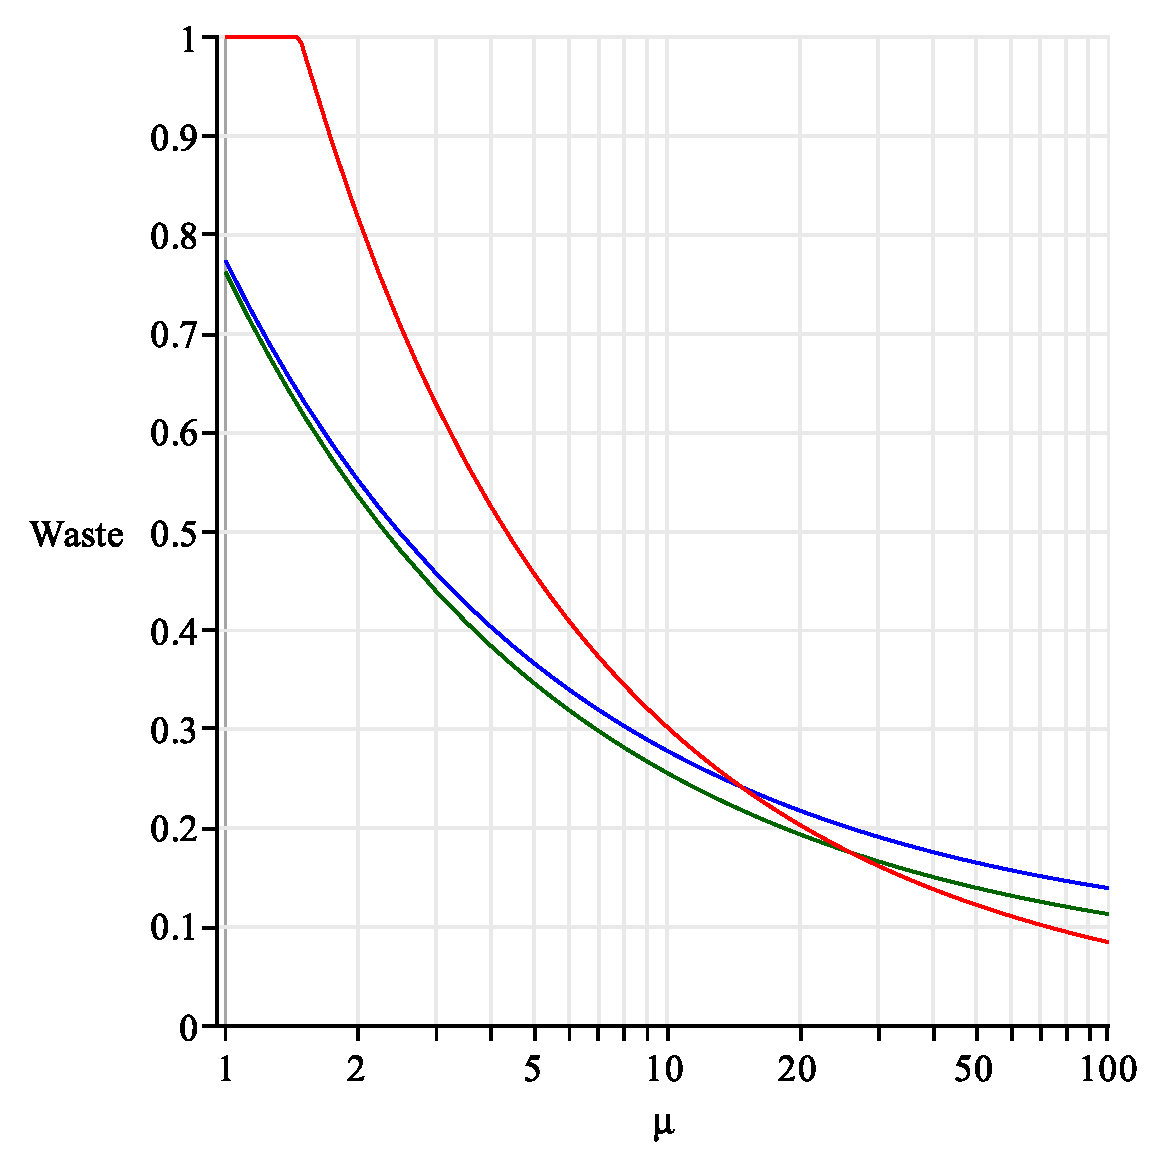
\includegraphics[width=0.3\textwidth,height=0.32\textheight,viewport=70 35 555 555,clip]{FatWasteMat100.pdf} &
  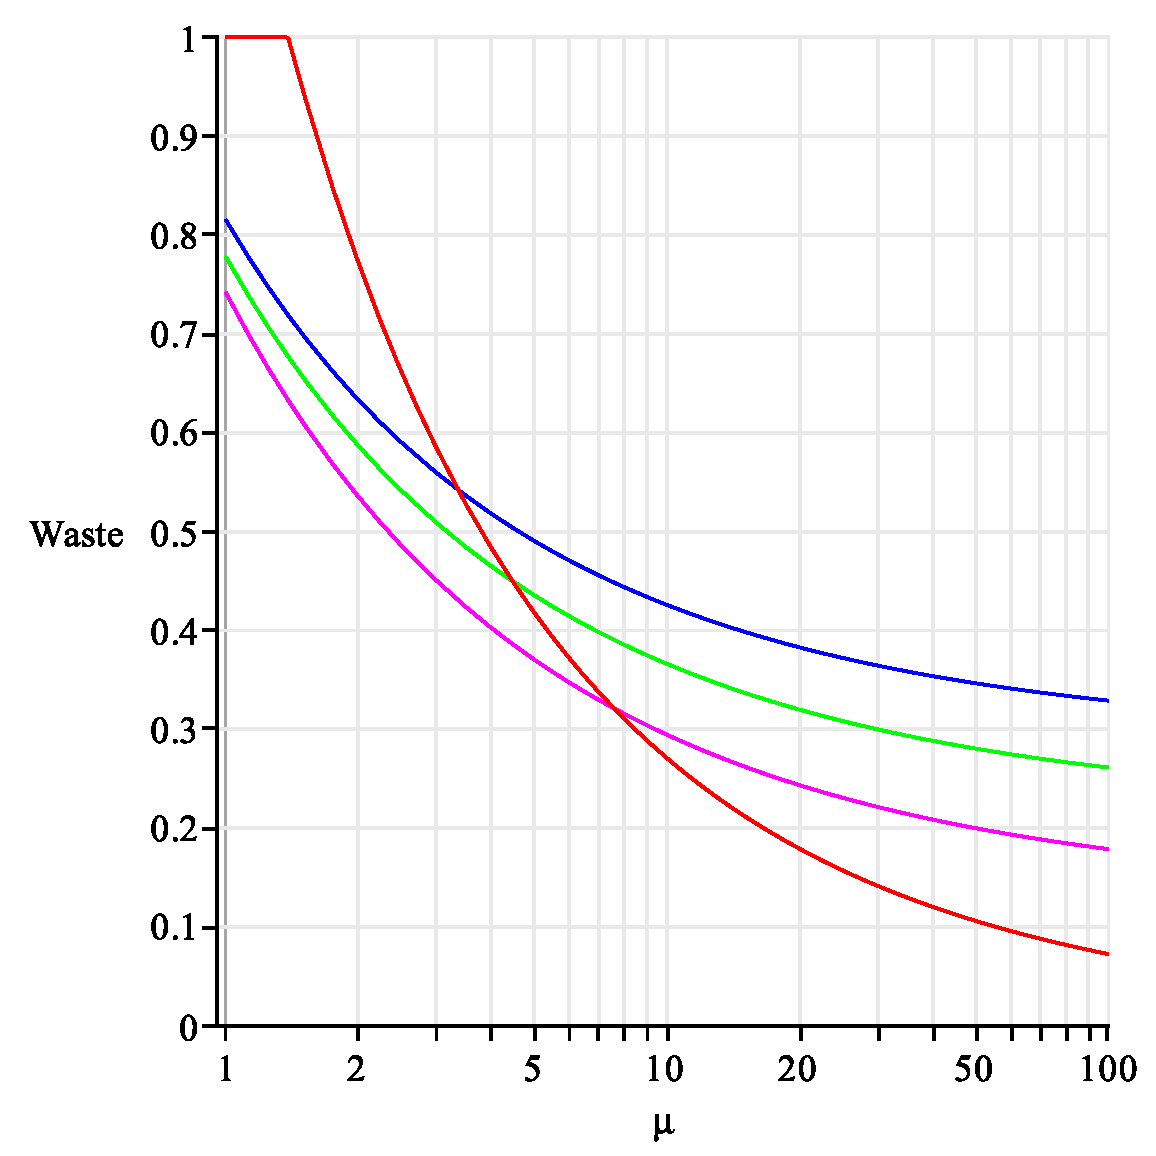
\includegraphics[width=0.3\textwidth,height=0.32\textheight,viewport=70 35 555 555,clip]{FatWasteStenc3D100.pdf} \\
 \end{tabular}
 ~\\
\centerline{Waste as a function of processor MTBF $\mu_{ind}$, $C=100$}
\end{frame}

\begin{frame}
  \frametitle{Conclusion on Hierarchical Checkpointing}

  \begin{itemize}
  \item Model for Hierarchical Checkpointing is \textcolor{red}{complex}
  \item Validation via simulation and comparison with few deployments
  \item \emph{All models are wrong, some are useful}
    \begin{itemize}
    \item Study highlights better resilience for \textcolor{blue}{fat} nodes for Exascale
    \item Narrow gap (\emph{application dependent}) of applicability for hierarchical approaches
    \end{itemize}
  \item Message Logging is doomed? See future work
  \end{itemize}
\end{frame}
